\documentclass[times,twocolumn,final]{elsarticle}

%% Stylefile to load MEDIMA template
\usepackage{medima}
\usepackage{framed,multirow}

%% The amssymb package provides various useful mathematical symbols
\usepackage{amssymb}
\usepackage{latexsym}

% Following three lines are needed for this document.
% If you are not loading colors or url, then these are
% not required.
\usepackage{url}
\usepackage{xcolor}

\usepackage{hyperref}

%%%%%
\usepackage{amsmath}
\usepackage[numbers]{natbib}
\usepackage{siunitx}
\usepackage{booktabs}
\usepackage{multirow}
%%%%%
\definecolor{newcolor}{rgb}{.8,.349,.1}

\newcommand{\xj}[1]{\textcolor[rgb]{1,0,0}{(#1)}}
\newcommand{\zj}[1]{\textcolor[rgb]{1,0,1}{(ZJ:#1)}}
\newcommand{\md}[1]{\textcolor[rgb]{0,0,1}{#1}}
\newcommand{\td}[1]{\textcolor[rgb]{0.5,0.0,0.5}{#1}}

\newcommand{\blk}{\mathbf{B}}
\newcommand{\nrt}{N}
\newcommand{\brc}{F}
\newcommand{\delete}[1]{}

\journal{Medical Image Analysis}

\begin{document}
	
\verso{Jie Zhao \textit{et~al.}}

\begin{frontmatter}

\title{Neuronal population reconstruction in ultra-scale optical microscopy images via progressive learning}                       
%\tnotetext[tnote1]{This is an example for title footnote coding.}

\author{Jie \snm{Zhao}}
\author{Xuejin \snm{Chen}\corref{cor1}}
\cortext[cor1]{Corresponding author: 
	Tel.: +86-551-63600852;  }
\ead{xjchen99@ustc.edu.cn}
%\fnref{fn1}}
%\fntext[fn1]{This is author footnote for second author.}
\author{Zhiwei \snm{Xiong}}
%% Third author's email
\author{Dong \snm{Liu}}
\author{Junjie  \snm{Zeng}}
\author{Yueyi \snm{Zhang}}
\author{Zheng-Jun \snm{Zha}}
\author{Guoqiang \snm{Bi}}
\author{Feng \snm{Wu}}

\address{National Engineering Laboratory for Brain-inspired Intelligence Technology and Application, University of Science and Technology of China, No. 96 Jinzhai Road, Hefei, Anhui, 230026, China} 


\begin{abstract}
Reconstruction of neuronal populations from ultra-scale optical microscopy (OM) images is essential to investigate neuronal circuits and brain mechanisms.
The noises, low contrast, huge memory requirement and high computational cost pose significant challenges in the neuronal population reconstruction.
%
Recently, many studies have been conducted to extract neuron signals using deep neural networks (DNNs).
However, training such DNNs usually relies on a huge amount of voxel-wise annotations in OM images, which are expensive in terms of both finance and labor.
%Moreover, the high memory cost of DNNs limits the volume of input images that can be handled at one time. 
%
In this paper, we propose a novel framework for dense neuronal population reconstruction in ultra-scale images.
%
To solve the problem of high cost in obtaining manual annotation for training DNNs, we propose a progressive learning scheme for neuronal population reconstruction (PLNPR) which does not require any manual annotations. 
%
Our PLNPR scheme consists of a traditional neuron tracing module and a deep segmentation network that mutually complement and progressively promote each other. 
%Based on the DNN model progressively trained, reconstructing neurons from local noisy image blocks is feasible with allowed memory.
%
To reconstruct dense neuronal populations in a terabyte-sized ultra-scale image, we introduce an automatic framework which adaptively traces neurons block by block and fuses multiple neurons in overlapped regions continuously and smoothly.
%
We build a dataset ``VISoR-40" which consists of 40 large-scale OM image blocks from cortical regions of a mouse.
Extensive experimental results on our VISoR-40 dataset and the public BigNeuron dataset demonstrate the effectiveness and superiority of our method on neuronal population reconstruction and single neuron reconstruction.
Furthermore, we successfully apply our method to reconstruct dense neuronal populations in a ultra-scale mouse brain slice. 
The proposed adaptive block-wise reconstruction and fusion strategy greatly improve the completeness of neurites in dense neuronal population reconstruction. 
\end{abstract}

\begin{keyword}
\KWD Neuronal population reconstruction 
\sep Ultra-scale images 
\sep Optical microscopy 
\sep Progressive learning
\end{keyword}

\end{frontmatter}


\section{Introduction}
\label{sec:introduction}

%Reconstruction of neuronal morphology is important for brain studies. 
Obtaining a blue print of the brain architecture, including the morphologies and interconnectivities of neuronal populations, allows for measuring and visualizing neuronal structure, understanding neuronal identity, and determining potential connectivity.
Therefore, complete reconstruction of neuronal populations from large-scale brain images is essential to investigate the mechanism of the nervous system, analyze brain changes, and facilitate our understanding of brain diseases such as dementia and Alzheimer's disease~\cite{Petrella2003, Giorgio2013}.
One of the key techniques in this endeavor is optical microscopy (OM), which allows detailed visualization of neurons and makes the reconstruction of every neuron possible~\cite{Senft2011}, as shown in Fig.~\ref{fig:brain}.
However, despite numerous efforts devoted, this task is still one of the main challenges in computational neuroscience.

\begin{figure}[t]
	\centering
	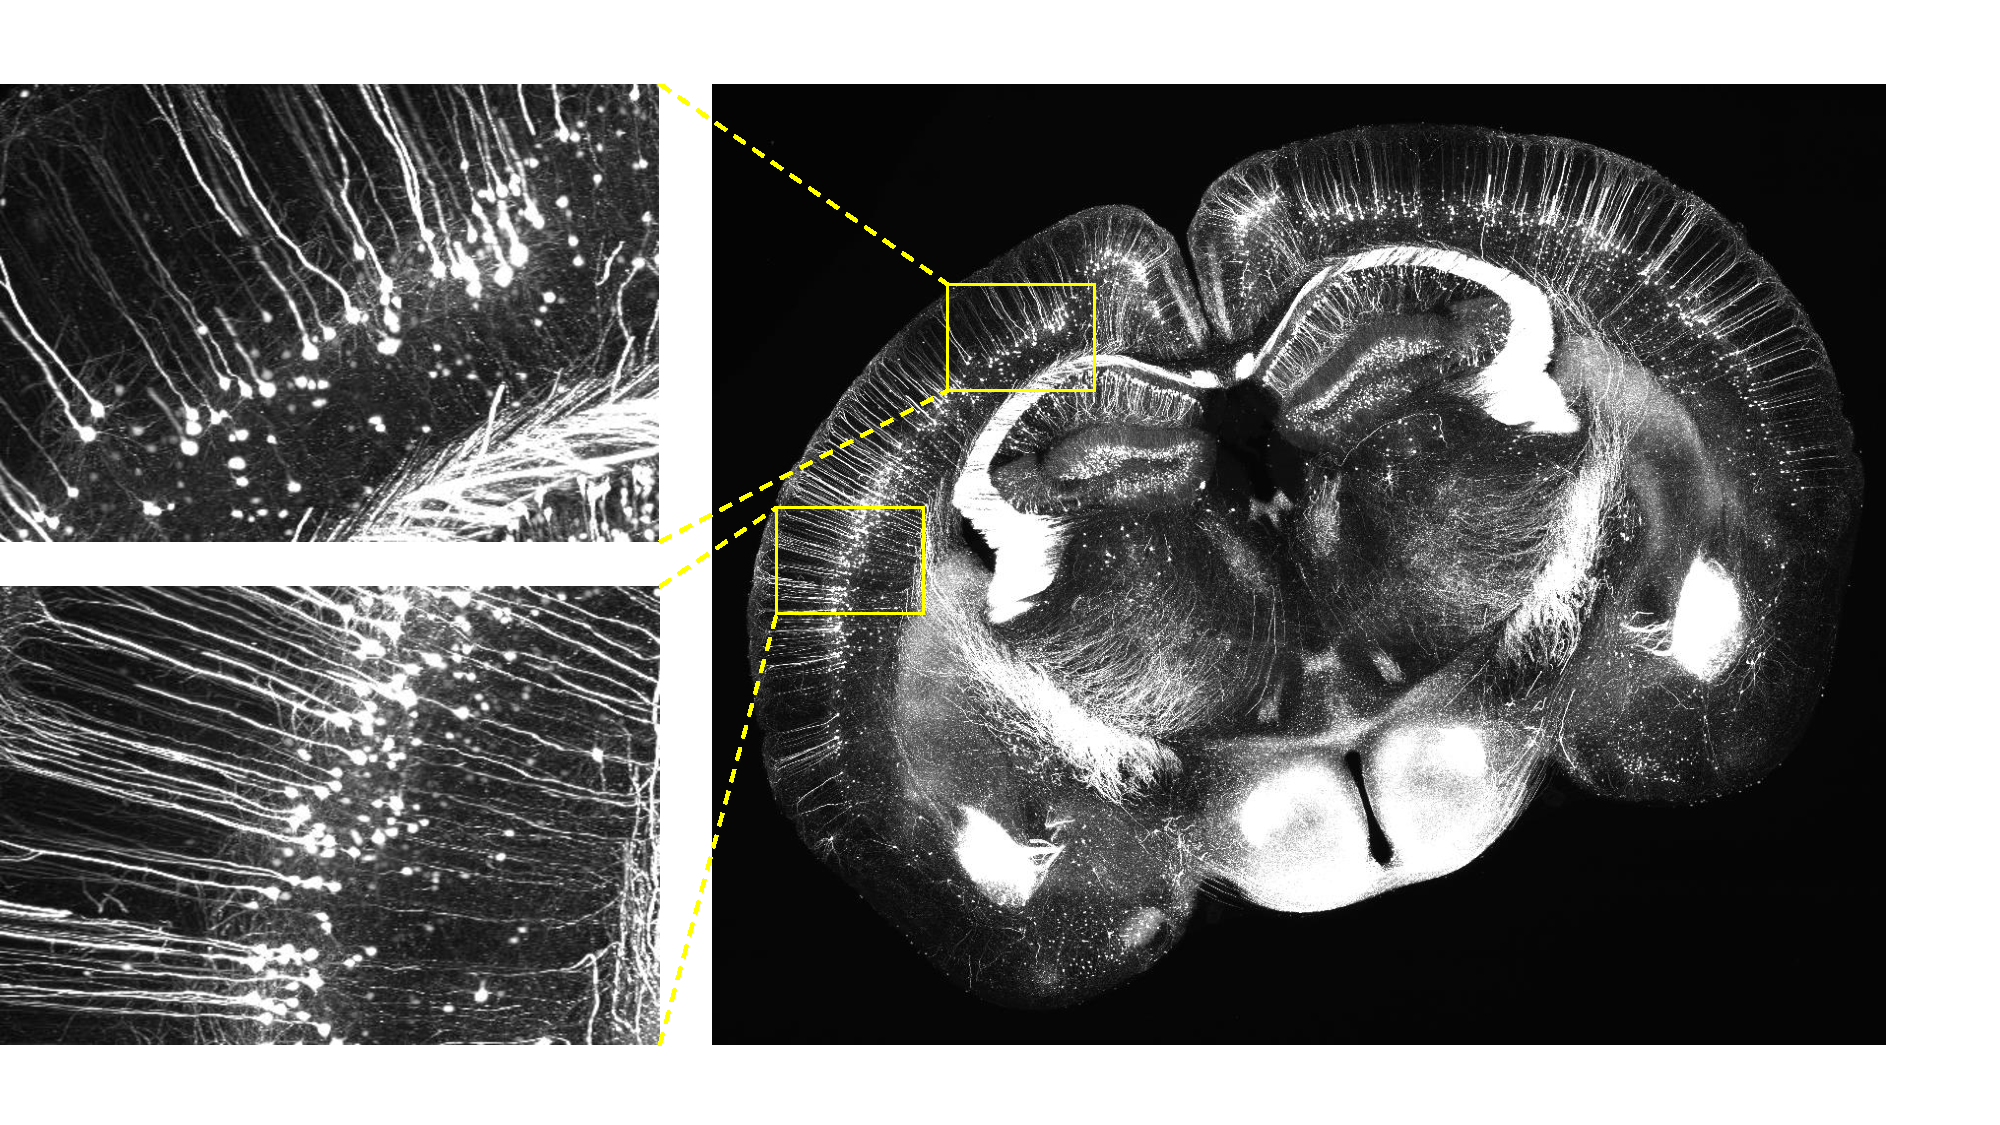
\includegraphics[width=1\columnwidth]{./Illustrations/brain2.pdf}
	\caption{A 3D mouse brain slice captured by the VISoR imaging system~\cite{Wang2019}. The dense neuronal populations, low contrast, image noises and large volume pose significant challenges for automatic reconstruction of neuronal populations from the ultra-scale image.}	
	%\caption{An image piece of a neuronal population in the neocortex of a whole mouse brain.}	  
	\label{fig:brain}
\end{figure}

The challenges in large-scale neuronal population reconstruction are mainly caused by complex morphology of neurons, low quality and large volume of OM brain images.
Due to the complicated process of imaging acquisition and the uneven distribution of fluorescence markers in neurons, the intensities of voxels that are occupied by neurons vary dramatically in highly noisy and inhomogeneous environments.
Moreover, to detail the structure of neurons in the brain, high resolution of OM images are required. Such an image typically contains trillions of voxels and the image size is formidably large in a terabyte scale. It is even impractical to directly load the entire large image into computer memory before reconstructing neurons when considering the memory cost and tracing time.
Manual reconstruction of neuronal populations from large-scale brain images is an extremely laborious and time-consuming task.
Sophisticated knowledge of neuron morphology is also required.
%
Therefore, an effective and automatic reconstruction algorithm for large-scale neuronal population in these challenging situations is greatly desired in practice.
 
 
Attempts have been made for neuron reconstruction for large-scale OM images in recent years, such as Neuron Crawler~\cite{Zhou2015}, \md{UltraTracer~\cite{Peng2017} and MEIT~\cite{Wang2018}}.
A common solution is to divide the large-scale image into blocks and trace neurons block by block.
Despite their great improvement in this task, several limitations still remain.


One main bottleneck is that the base tracers used for neuron tracing in image blocks typically \md{employ a series of traditional image processing algorithms such as binarinzation, fast marching, fusion, etc. }
Unfortunately, these algorithms using hand-crafted features and rules have difficulty in reconstructing neurons from low-contrast and noisy image blocks.
To improve the reconstruction quality, deep learning techniques have been adopted in neuron reconstruction recently~\cite{Xu2016, Li2017, Zhou2018}. 
However, these approaches require huge amount of manually annotated data for neuron segmentation network training.
%
We observe that the reconstruction maps inferred from existing conventional algorithms can effectively provide approximate locations of neurons. 
Although these voxels may not cover all neurons, they still provide important cues for obtaining complicated patterns of neurons.
Therefore, we propose a progressive learning scheme for neuronal population reconstruction (PLNPR) to take advantage of both conventional methods and deep learning techniques.
More specifically, we employ conventional methods to produce pseudo-labels to train a deep segmentation network. 
The network is expected to learn more comprehensive features of neurons from noisy labels. 
With a more powerful network for segmenting neurons, the neuron reconstruction using conventional tracers could be improved. 
Then we progressively refine the network with better neuron reconstruction results as pseudo labels, and reconstruct more complete neurons with better neuron segmentation.
We first investigate this concept in our preliminary work \cite{Zhao2019} on a few image blocks. 
In this work, we apply PLNPR on dense neuron population reconstruction in a ultra-scale OM image slice. 

Another bottleneck of existing large-scale neuron reconstruction methods~\cite{Zhou2015, Peng2017, Wang2018} is that they mainly focus on single neuron reconstruction. 
%
For dense neuronal population reconstruction in large-scale OM images, dense neurites may cross with each other, which makes the neuron tracing much more challenging in low-contrast and noisy OM images. 
% 
Following the commonly used block-by-block framework, we introduce UltraNPR, which utilizes our PLNPR approach as the base tracer in blocks, and \md{design a novel tracing strategy with a fusion algorithm  for dense neuronal populations}.
%
\xj{Describe the main idea, the difference from existing tracing methods in the technical aspect. }


%In this work, we introduce UltraNPR, an algorithm designed for reconstructing dense neuronal populations from large-scale or even ultra-large-scale images. UltraNPR reconstructs neuronal populations by progressively improving the completeness of neuronal structure block by block.
%
\delete{Firstly, the large-scale raw image is divided into blocks of the same size.
Since somas are where signals from the dendrites are joined and pass on, UltraNPR begins the reconstruction from the blocks that contain somas.
% which can be detected using existing soma detection methods.
For robust reconstruction from low-quality images, our PLNPR method is applied to trace neurons in each block.
Based on the reconstruction results in already-reconstructed blocks, UltraNPR automatically and adaptively searches the next block to trace.
%For each block containing somas, this reconstruction procedure repeats until no new terminal tips could be detected or the next block contains somas.
%Finally, UltraNPR analyzes the reconstruction results in all blocks, and assembles the matched neurites from adjacent blocks to obtain the final complete neuronal population reconstruction. In our implementation, 
Finally, a fusion algorithm is designed to make the fragmented neurites of a neuron from adjacent blocks can be assembled continuously and smoothly.
In this way, UltraNPR is capable of exploring a large-scale image for neuronal population reconstruction.
}


%%%%%%%%%%%%%%%%%%%%%%%%%%%%%%%%%%%%%%%
In summary, we make the following contributions in this work. 
\begin{enumerate}
\item We propose a general progressive learning framework that can integrate existing neuron tracing and deep segmentation networks for neuron reconstruction without using manual annotations.

\item We integrate our PLNPR with a block-wise propagation and fusion strategy which can reconstruct dense neuronal populations from trillions of voxels in an image slice. 

\item We build a dataset ``VISoR-40" which consists of 40 OM image blocks from mouse cortical regions. Manual annotations of eight blocks in the dataset are available. 
%which consists of 40 OM images from mouse cortical regions and contains about 400 neuronal trees. Publishing this dataset will strongly support the study of deep neural networks for microscopic explorations.
\item Extensive experiments on our VISoR-40 dataset and the public BigNeuron dataset demonstrate the effectiveness and superiority of our progressive learning algorithm for both neuronal population reconstruction and single neuron reconstruction.
\end{enumerate}

%%%%%%%%%%%%%%%%%%%%%
%Before proceeding into the detailed account of our approach, it is useful to briefly review the related research efforts.
\delete{
The remainder of this paper is organized as follows. In Section~\ref{sec:related work}, we make a survey of related work. In Section~\ref{sec:method}, we first introduce the PLNPR algorithm, then elaborate the UltraNPR algorithm. We report the experiment results and discussions in Section~\ref{sec:experiments}. Finally, conclusions are drawn in Section~\ref{sec:conclusion}.
}
\section{Related Work}
\label{sec:related work}
\begin{figure*}[ht]
	\centering
	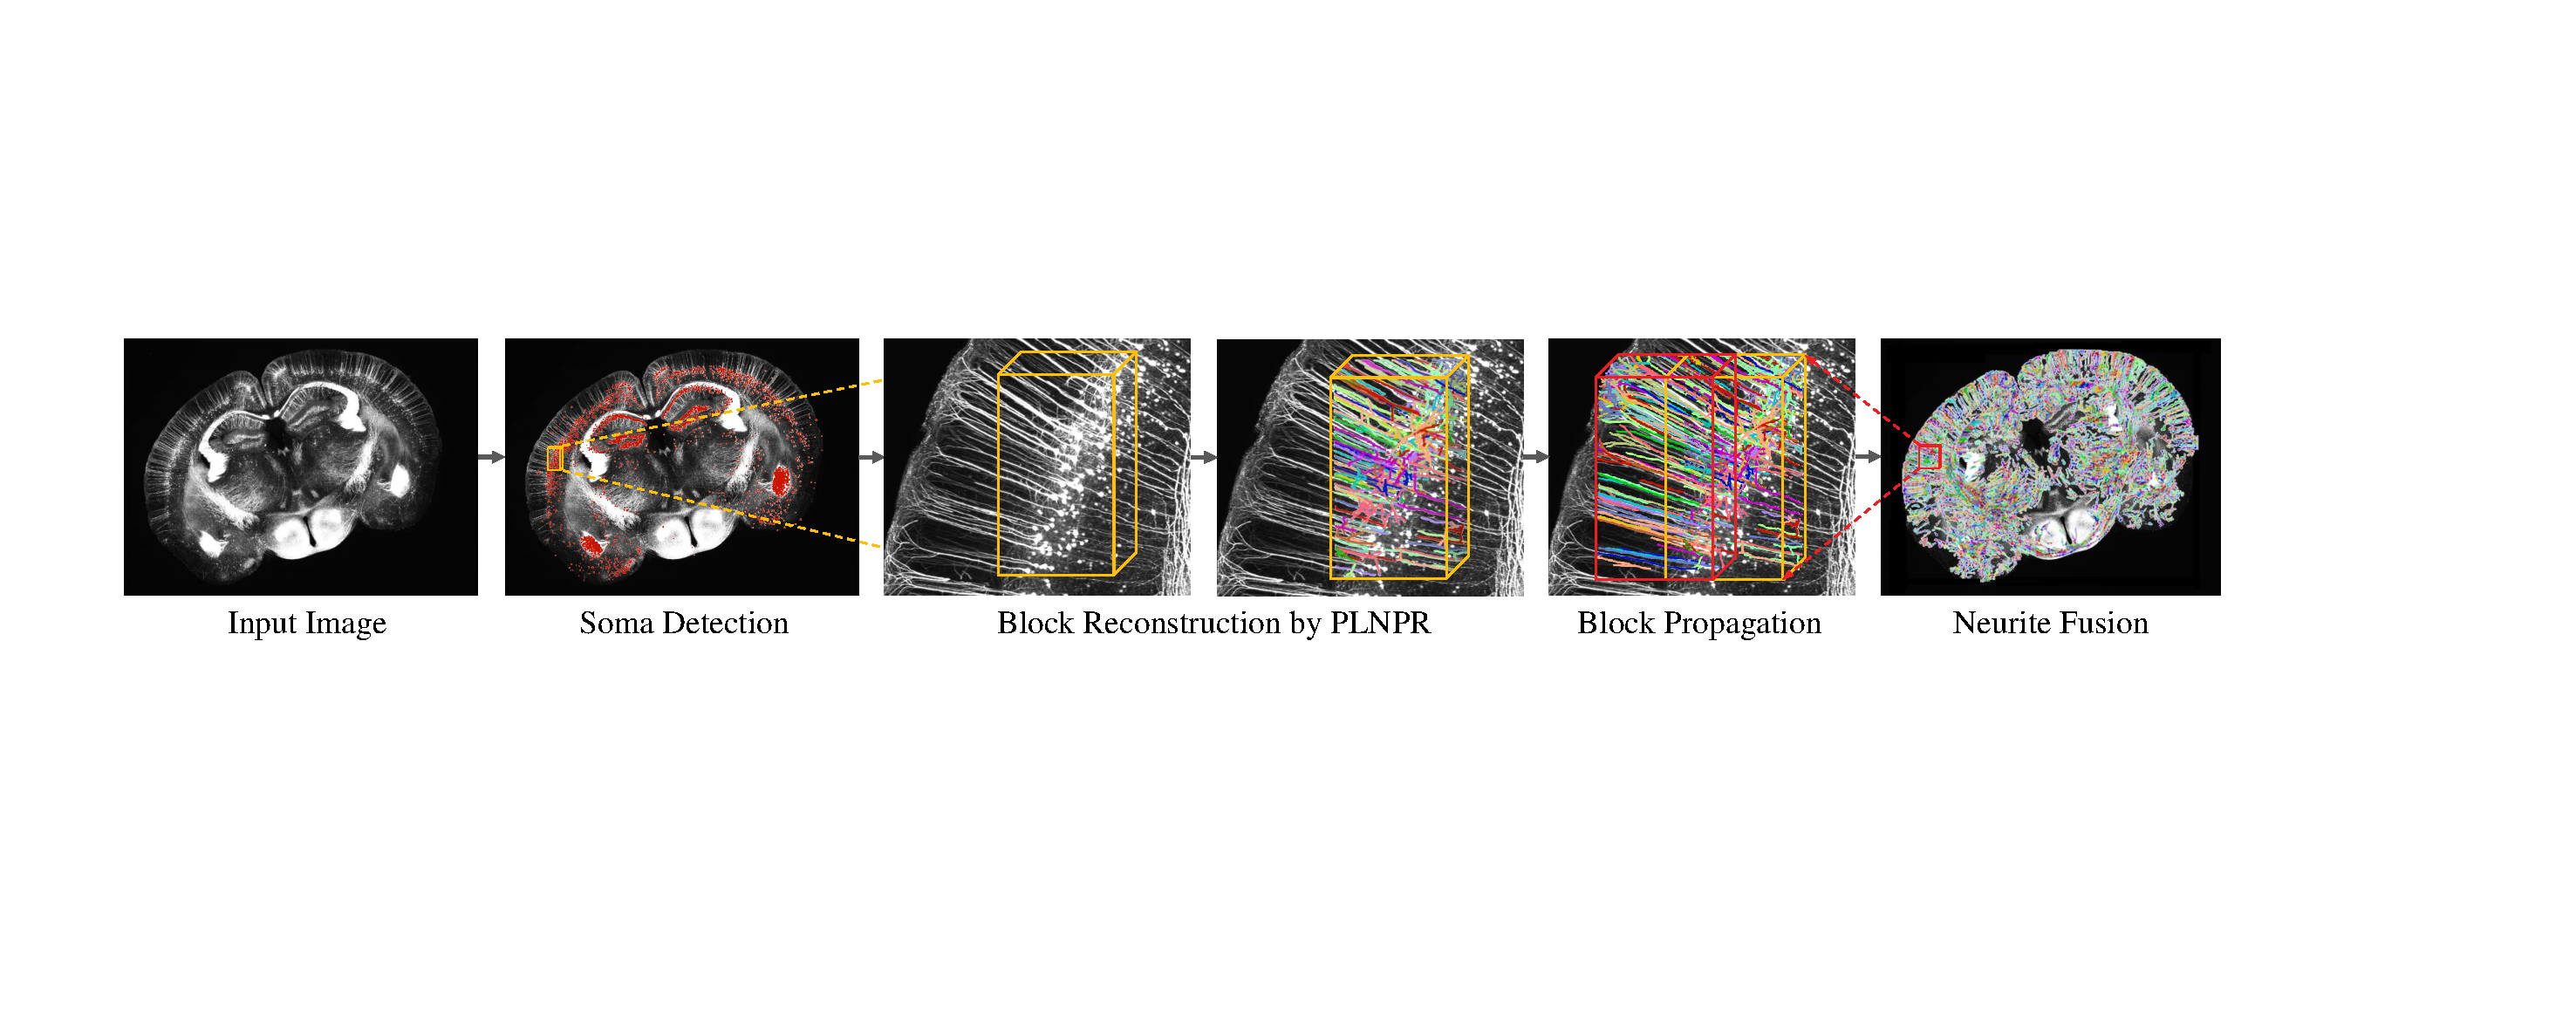
\includegraphics[width=1\textwidth]{./Illustrations/framework_ultranpr.pdf}
	\caption{Diagram of our UltraNPR algorithm for neuronal population reconstruction from an ultra-scale image of a brain slice.}
	\label{fig:ultra_framework}
\end{figure*}

%\subsection{Techniques for Robust Neuron Reconstruction}
%\label{sec:neuron reconstruction}

Early techniques for neuron reconstruction from optical microscopy images typically employ traditional image processing algorithms, such as snakes~\cite{Wang2011, Cai2006}, principal curves~\cite{Bas2011}, graph theory~\cite{Peng2010a, Yang2013, De2016}, model-fitting~\cite{Zhao2011, Santamaria2015}, watershed~\cite{Navlakha2013, Suembuel2016}, energy minimization~\cite{Quan2013, Liu2016}, mean-shift clustering~\cite{Frasconi2014}, ray-shooting~\cite{Wu2014, Liu2019}, fast-marching~\cite{Peng2011, Xiao2013, Liu2018}, and so on.
Unfortunately, these conventional algorithms rely on hand-crafted features and carefully tuned parameters, thus usually tending to fail when the image quality is poor.
%TReMAP~\cite{Zhou2016}, NGPST~\cite{Quan2015},

To improve the reconstruction performance from low-quality image blocks, many machine learning techniques have been introduced to extract neuron voxels from noisy and low-contrast images for further reconstruction. 
This kind of methods employs various classifiers with hand-crafted features, such as support vector machine (SVM)~\cite{Chen2015}, minimum spanning tree~\cite{Basu2016}, Bayesian probabilistic model~\cite{Radojevic2017}, Bootstrap aggregating~\cite{Wang2017}, gradient boosting decision trees (GBDT)~\cite{Gu2017}, Markov chain Monte Carlo (MCMC)~\cite{Skibbe2015, Skibbe2019}, and so on.
However, these methods employ hand-crafted features that usually suffer from limited representation capability for accurate recognition, considering more challenging images and complex neuron morphologies.


Recently, deep-learning-based methods~\cite{Li2017, Zhou2018, Xu2016, Kozinski-MIA2020} bring the power of DNNs to improve the reconstruction performance. 
Instead of manually designing sophisticated features, these DNNs learn feature representations in a data-driven way and extract more distinctive features. 
With more powerful feature representation and classifiers for extracting neurons from image blocks, these methods achieve more robust reconstruction results. 
Despite great improvements, these DNN-based methods rely on extensive manual annotations of neuron voxels for network training.
Unfortunately, due to the complicated morphology of neurons and the low quality of OM images, such annotations are very costly to obtain in terms of both time and labor.
%
In comparison, we propose a novel iterative framework to progressively improve the DNN-based neuron reconstruction performance without using manual annotations.


%\subsection{Large-scale Neuron Reconstruction}
%\label{sec:largescale}

%Most existing neuron reconstruction methods focus on robust and accuracy neuron reconstruction from small-size noisy image blocks. 
Despite substantial advancements brought by existing methods, they often need to load all the voxels into memory before neuron tracing.
The sheer volume of an ultra-scale OM image is usually far beyond the processing capability, especially on the memory cost and tracing time.
%
In recent years, some attempts have been made to reconstruct neurons from large-scale OM images, such as Neuron Crawler~\cite{Zhou2015}, UltraTracer~\cite{Peng2017}, and MEIT~\cite{Wang2018}.
To tackle the challenge of huge image volume, a common solution is to reconstruct a neuron block by block. 
%Each block is cropped from the raw image and is much smaller in size than the raw image.
In each local block cropped from a large-scale image, existing tracing methods, such as APP2~\cite{Xiao2013}, MOST~\cite{Wu2014}, and FMST~\cite{Yang2019}, can be directly used as the base tracer to trace neurites. 
Starting from the cell body, the neurites are then traced in neighboring blocks and then fused together based on signal strengths and structure continuity.
%
However, all of these methods focus on single neuron reconstruction.
The input images usually contain only one single neuron so that the signal is very sparse without confusion of different neurons. 
%
In comparison, we target a more challenging task to reconstruct dense neuronal populations from ultra-scale OM images, where closely spaced neurites that belong to different neurons are difficult to distinguish for existing methods that are designed for single neuron reconstruction.


\section{Proposed Method}
\label{sec:method}
\begin{figure*}[th]
	\centering
	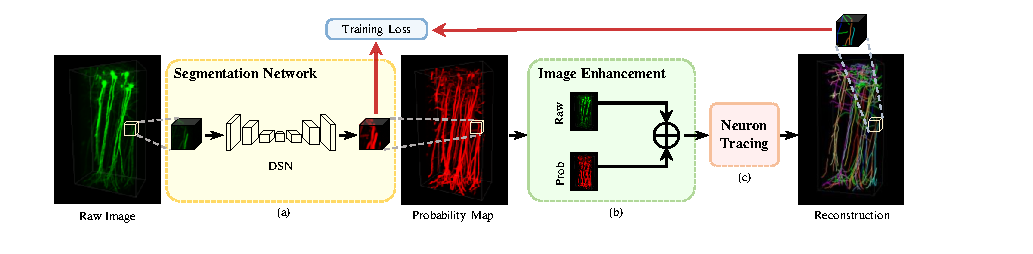
\includegraphics[width=1\textwidth]{./Illustrations/framework_plnpr.pdf}
	\caption{Diagram of our progressive learning algorithm for neuron reconstruction from an image block. (a) The segmentation network extracts neuron signals from the raw image. (b) The output probability map is employed to enhance the raw image in order to preserve both global structures and local signal details, which facilitates the neuron tracing module (c) for more complete neuronal population reconstruction. To train the segmentation network, we use the reconstructed neurons as pseudo labels (red arrows), and iteratively refine the network model and neuron reconstruction with a set of images. The black arrows show the reconstruction pass from an image block at the test stage.}
	\label{fig:framework}
\end{figure*}


Given an ultra-scale noisy OM image, our UltraNPR follows a block-by-block neruon reconstruction scheme, as Fig.~\ref{fig:ultra_framework} shows. 
%
The ultra-scale input image may contain billions or even trillions of voxels.
We first divide the input image into blocks that are averagely in size of $0.5mm\times 1mm\times 0.4mm$ with overlaps. 
%
For each block, we first enhance the noisy images by a deep neural network, which is progressively trained from reconstructed neurons using our PLNPR. 
Then we reconstruct neuronal populations in each block using the enhanced image. 
%
Since it is more reliable to start from somas rather than subtle neurites for neuron reconstruction, we first detect somas and start tracing from the blocks where somas can be detected. 
%
Our UltraNPR then employs an effective block propagation strategy to trace dense neuronal populations in an adaptive order by finding neighboring blocks with more neurite tips. 
Finally, we fuse overlapped neurites in adjacent blocks to reconstruct complete neuronal populations from the whole ultra-scale image.


\subsection{PLNPR for Robust Neuron Reconstruction}
%\subsection{Unsupervised Progressive Learning for Neuronal Population Reconstruction}
\label{sec:PLNPR}

To reconstruct neurons from a noisy OM image block, our PLNPR algorithm consists of three key components: a segmentation network, an image enhancement module, and a neuron tracing module, as shown in Fig.~\ref{fig:framework}. 
%
The segmentation network is designed to extract neuron voxels from noisy and complex backgrounds.
Compared with existing segmentation networks that are trained with dense voxel-wise annotations for strong supervision, we use pseudo labels that are generated using traditional neuron tracing methods.
%
In each iteration of segmentation and reconstruction, we apply the NGPST~\cite{Quan2015} as the neuron tracing module to reconstruct neurons from image blocks. 
The tracing module can be replaced by any other tracing method that does not require manual annotations for training.
%
It takes an image block $\mathbf{B}$ as input and reconstructs a neuronal population with separated neurons.
%The intensity $\mathbf{I}(x)$ of a voxel $x$ belongs to $[0,1]$.
From the reconstruction results, we produce a binary mask $\mathbf{M}$ indicating foreground by $\mathbf{M}(x)=1$ and background by $\mathbf{M}(x)=0$ for a voxel $x$.


Given $N$ unlabeled image blocks, we train our segmentation network using the neuron masks $\{\mathbf{M}_i\}_{i=1}^{N}$ generated from the neuron tracing module.
%
The output of the neuron segmentation network is a 3D probability map $\mathbf{P}$, which is computed by a voxel-wise softmax activation function. $\mathbf{P}(x)\in [0,1]$ indicating the probability of a voxel $x$ to be a neuron part.
%
Then, by fusing the predicted probability map with the raw image signals, the image block is enhanced in order to preserve both local signals and global structures simultaneously.
When the enhanced block is fed into the neuron tracing module, more complete neuronal populations can be reconstructed and provide better pseudo labels for the next iteration of network training. 
%
Based on the iterative learning process, the DNN and neuron tracer mutually complement and promote each other to gradually improve the neuron reconstruction performance.


 

\subsubsection{DNN for 3D Neuron Segmentation}
\label{sec:network}
 
Extracting neuron voxels from image blocks is non-trivial since the size, morphology, and intensity of neurons vary significantly.
In recent years, many 3D DNNs, such as 3D U-Net~\cite{Cicek2016}, 3D DSN~\cite{Dou2017}, and DenseVoxNet~\cite{Yu2017}, have demonstrated their outstanding capability in various biological and biomedical image segmentation tasks.
%
We extend the 3D DSN~\cite{Dou2017} as our neuron segmentation network to balance the performance and computation burden.
%
Although the original 3D DSN has achieved excellent performance for 3D organ segmentation~\cite{Dou2017}, it is prone to overfit in our case due to the limited training data. 
We employ the dropout~\cite{Srivastava2014} technique during training to learn more robust features that better generalize to new data.
In each convolutional layer, the dropout with a rate of $0.5$ is applied.% in our network. 


Another challenge in training 3D DNN is the memory limitation because the 3D feature images are huge with respect to the input size. Therefore, for each input image block, we crop a group of small cubes in size of $160\times 160\times 160$ with $30\%$ overlaps, and set batch size to 1 during training. 
%
To have the same physical resolution with the lateral dimension in OM image blocks, voxels in the axial dimension are interpolated after the imaging process. However, this interpolation leads to inhomogeneous image quality along different dimensions. 
Therefore, a random transposition process is employed for each cube as data augmentation for network training.

%Correspondingly, at the test time, we stitch these overlapped probability cubes together using average blending to get a probability map in the same size with the input block.

In addition, the volume of neuron voxels is usually much smaller than that of background in an OM image.
A data balancing technique is employed for network training.
When computing the training loss, we only consider the neuron voxels and a certain portion of background, which is randomly selected as non-neuron samples.
The number of non-neuron voxels used for training is set as $10$ times that of neuron voxels.


\subsubsection{Image Enhancement}
\label{sec:enhancement}

After training the segmentation network using pseudo labels, the trained model is used to predict a probability map for each image cube. 
By averaging the probabilities of the overlapped voxels between adjacent cubes, we can obtain the probability map $\mathbf{P}$ for the entire block $\mathbf{B}$.
Each element in $\mathbf{P}$ indicates the probability of the corresponding voxel in $\mathbf{B}$ being a neuron voxel.
To utilize the probability map, one natural way is to reconstruct neurons directly from it.
However, since the pseudo labels are not as accurate as manual annotations, especially at the early iterations, some local details might lose in the probability map. Therefore, we employ an enhanced representation by fusing the probability map and the raw image block in order to keep detailed structures and suppress noise signals effectively.
Specifically, a new probability map $\widetilde{\mathbf{P}} $ is first constructed by linearly mapping the value range of $ \mathbf{P}\in [0,1] $ to the value range $[{b}_{min}, {b}_{max}]$ of $\mathbf{B}$ as
\begin{equation}
\widetilde{\mathbf{P}}(x) = ({b}_{max}-{b}_{min})\mathbf{P}(x).
\end{equation}
%
Then, an enhanced block $\mathbf{E}$ is computed as
\begin{equation}
\mathbf{E}(x) = \alpha\widetilde{\mathbf{P}}(x) + (1-\alpha)\mathbf{B}(x),
\label{equ: enhance}
\end{equation}
where $\alpha\in [0,1]$ is a weight to control the contributions of voxel $ x $ in the original intensity and the probability map. By feeding the enhanced block to the neuron tracing module, neuronal populations can be reconstructed more completely.


With more reliable reconstruction results as pseudo labels, the segmentation network could be further trained to learn more discriminative and representative features for producing probability maps, which in turn benefit the tracing module to reconstruct more complete neurons in the next iteration.
%
As shown in Fig.~\ref{fig:ngps} (a), a raw image block typically contains many noises and inhomogeneous intensities.
At first, by feeding the raw block to the tracer~\cite{Quan2015}, the reconstructed neuronal population is incomplete and many neurites are missing, as Fig.~\ref{fig:ngps}(g) shows, comparing with the ground truth (GT) shown in Fig.~\ref{fig:ngps}(k).
%
Then, by utilizing the pseudo labels derived from imperfect reconstruction, the segmentation network can be trained to learn features for global morphology. Fig.~\ref{fig:ngps}(b) shows the predicted probability map, which demonstrates the enhanced trajectories.
With more iterations of neuron reconstruction and network training, more distinctive and long-range trajectory features can be progressively captured by the network, as shown in Fig.~\ref{fig:ngps}(c)(d)(e).
By combining the original image intensities with the predicted probability map, both local signal details and global trajectories are well preserved in the enhanced block, as Fig.~\ref{fig:ngps}(f) shows.
Iteration by iteration, the completeness and accuracy of neuron reconstruction are progressively improved, as shown in Fig.~\ref{fig:ngps}~(h)(i)(j).


\begin{figure}[t]
	\centering
	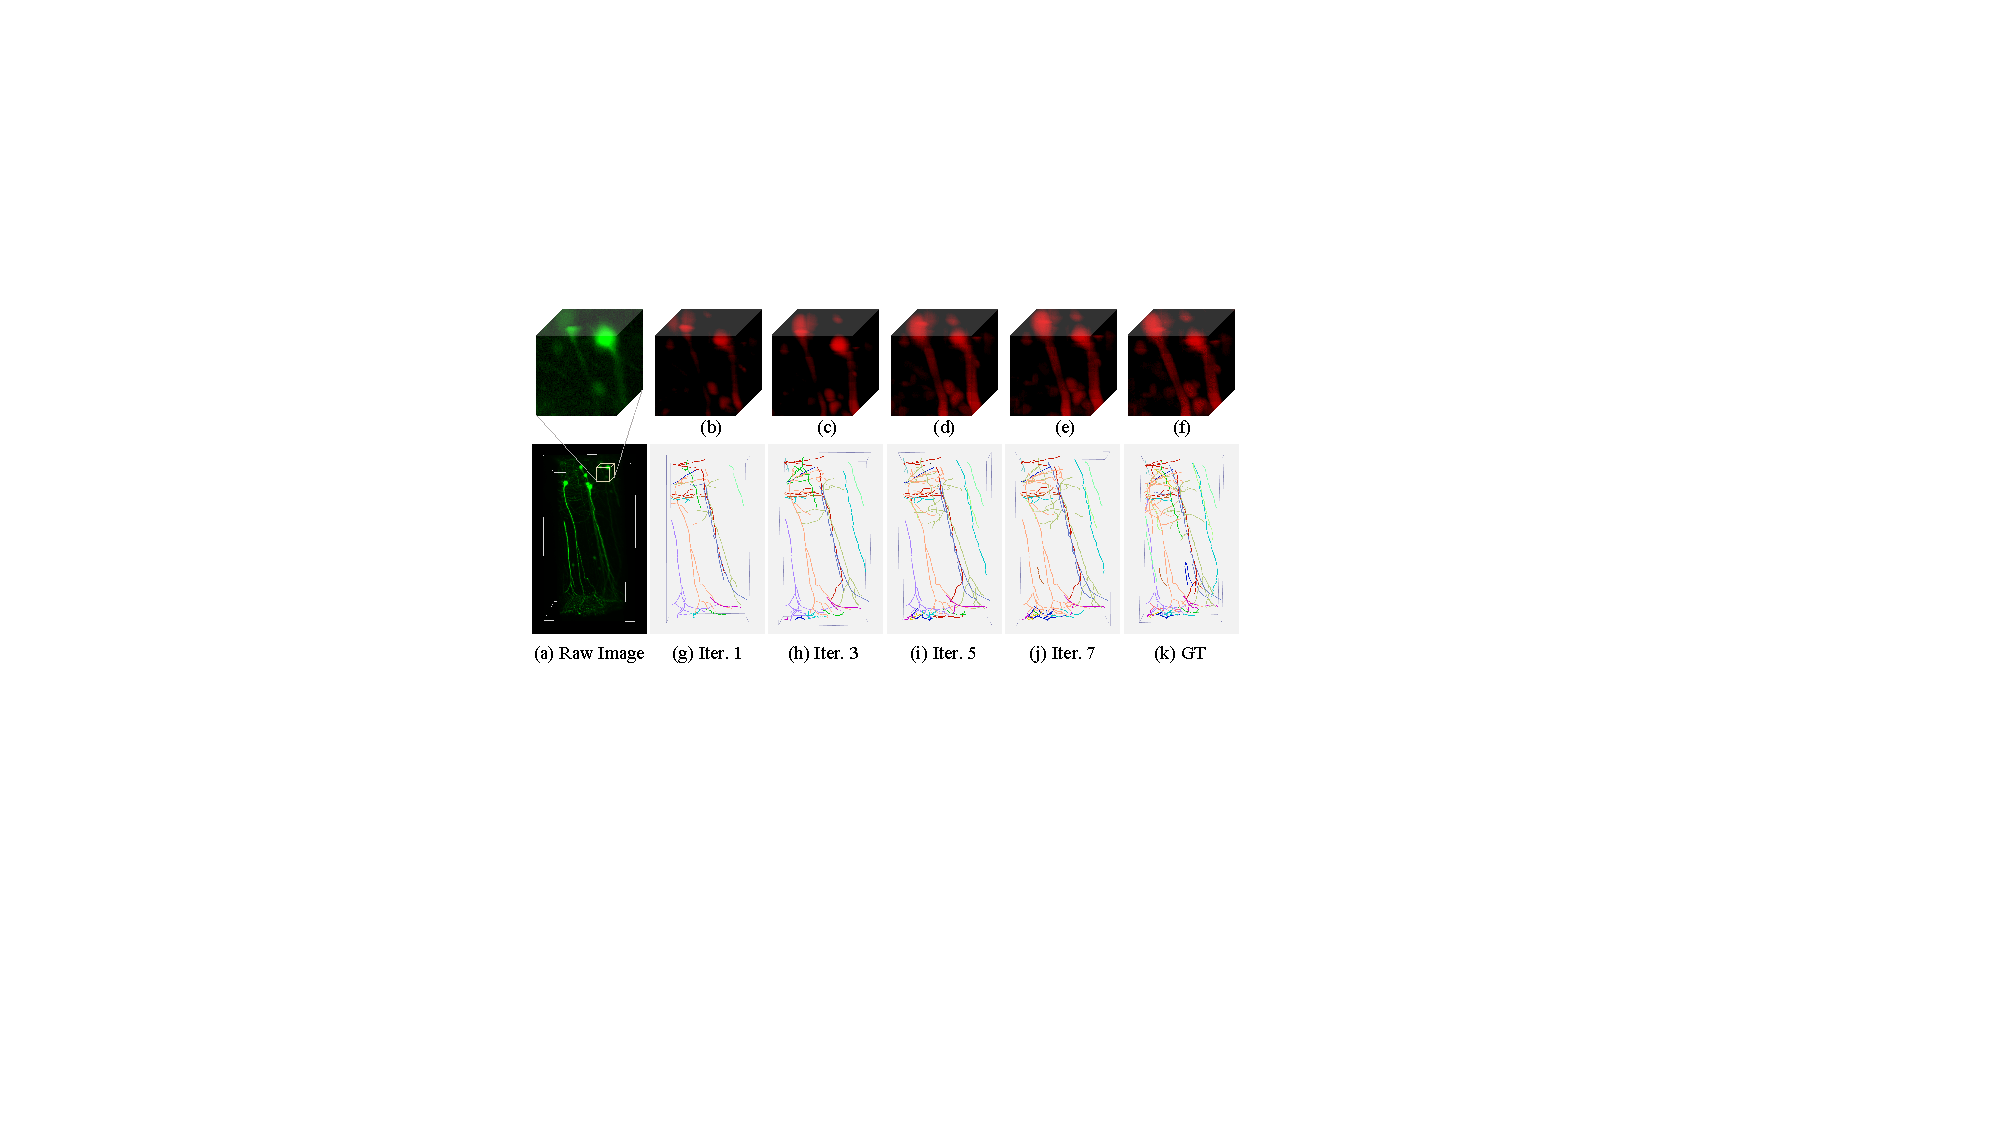
\includegraphics[width=1\columnwidth]{./Illustrations/ngps.pdf}
	\caption{Our progressive learning technique gradually improves the segmentation network to extract neuron signals from a raw image block (a). 
	(b-f) The probability maps generated by the segmentation network at different iterations.
		%Combing the probability map and the raw intensity, the enhanced block preserves both global trajectory and local details. 
	(g-j) More and more complete and accurate reconstruction of the neuronal populations can be obtained with more iterations. (k) Manually labeled neurons. Separated neurons are shown in different colors.}
	\label{fig:ngps}
\end{figure}
%

\subsection{Ultra-scale Neuronal Population Reconstruction}
\label{sec:UltraNPR}

\begin{figure}[t]
	\centering
	%\vspace{1cm}
	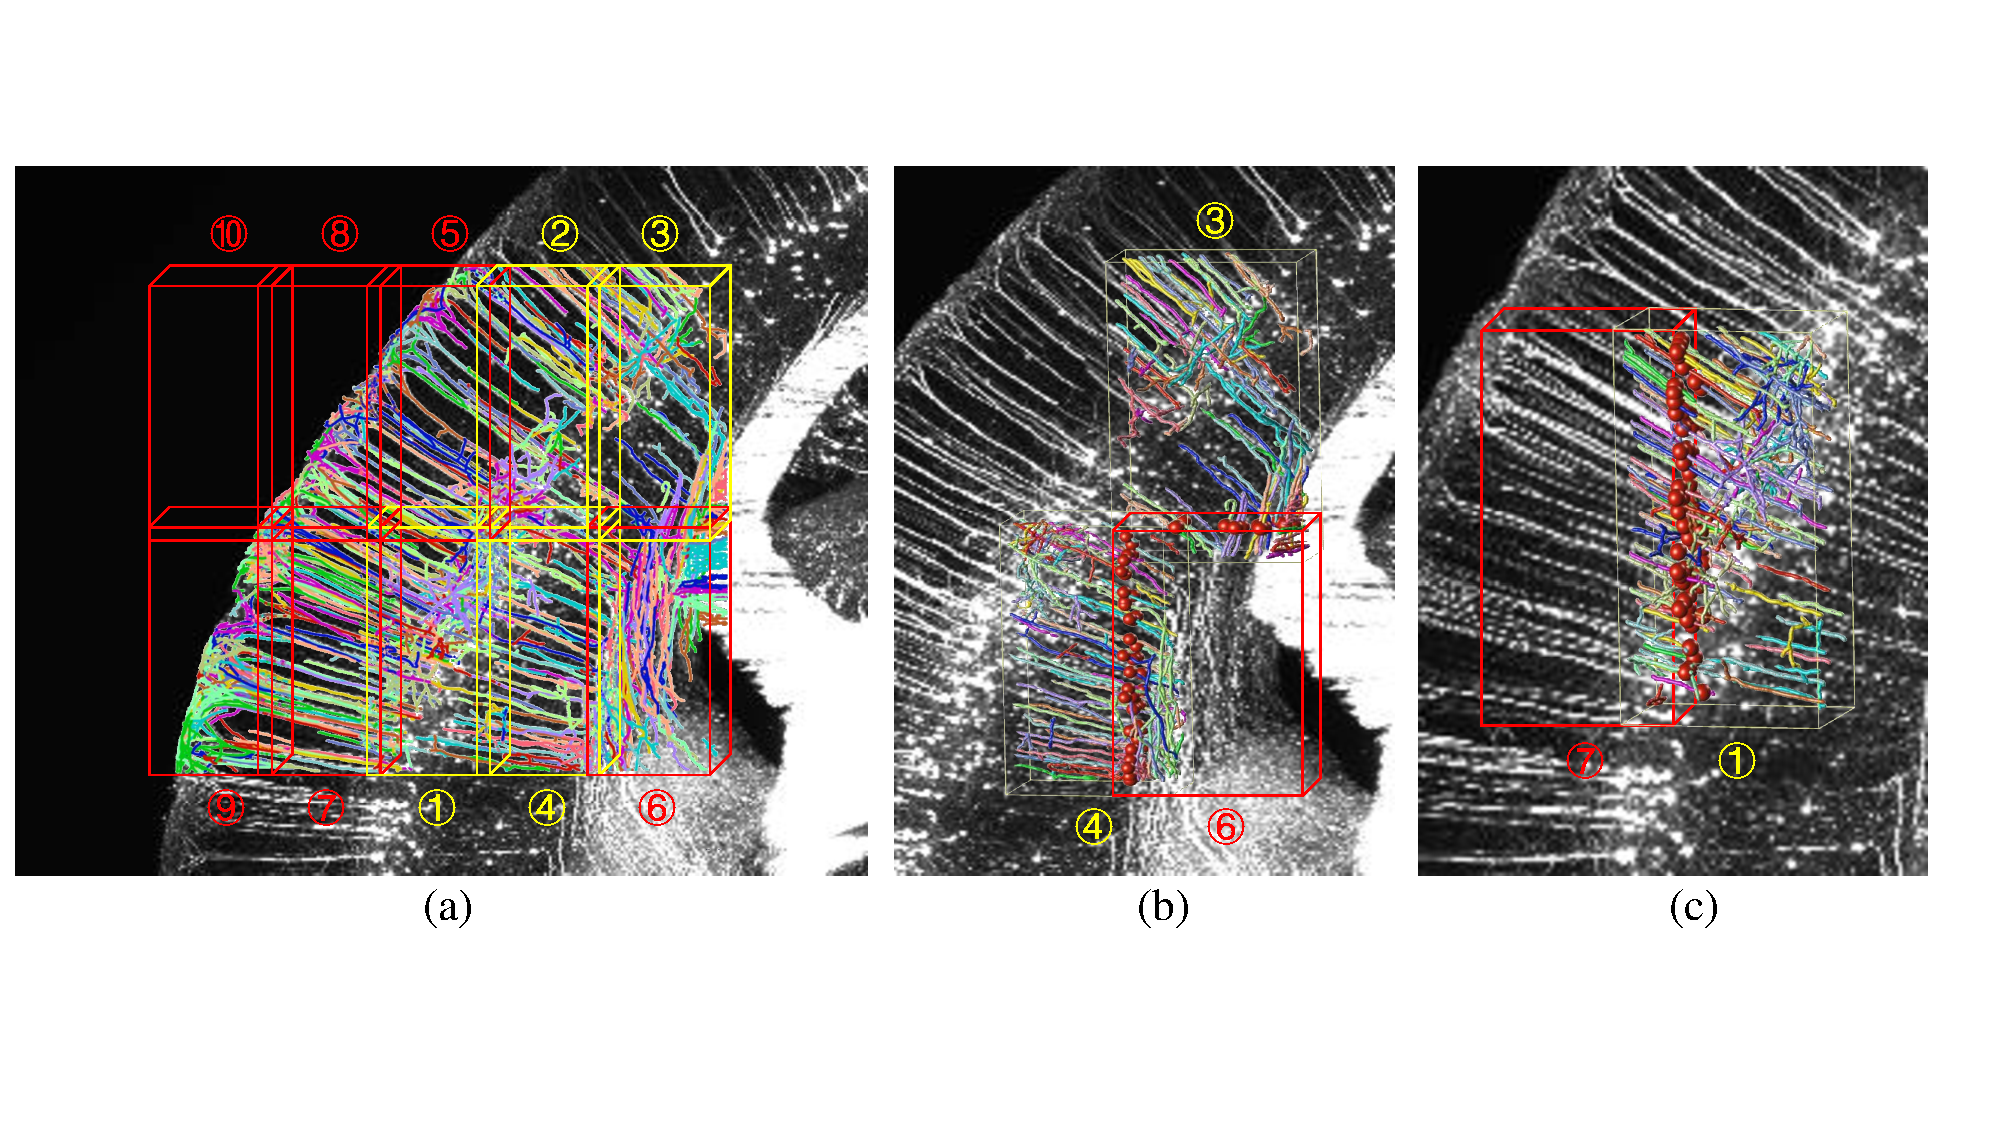
\includegraphics[width=1\columnwidth]{./Illustrations/ultranpr_block_search.pdf}
	\caption{An example of the iterative block reconstruction for ten blocks. (a) The number indicate the order in which the ten blocks are traced. The blocks 1, 2, 3, 4 are firstly reconstructed using our PLNPR since there are somas detected in these four blocks. (b) Block-6 is reconstructed by setting the neurite tips (red dots) from its two neighboring blocks (3, 4) as pseudo somas for tracing. (c) Block-7 is reconstructed by setting the neurite tips from its neighboring block-1 as pseudo somas.}
	\label{fig:blocksearch}
\end{figure}


Our PLNPR enhances the image signals and traces neurons from each image block.
However, neurons usually exist across multiple blocks in an ultra-scale image. 
% 
We propose an effective stitching process by looking for the most continuous block to trace dense neuron populations from all unreconstructed blocks. 
%
As somas are where signals from the dendrites are joined and pass on, we start from reconstructing neurons in the blocks where somas can be detected.
For blocks where no soma can be detected, we trace the neurons by generating pseudo-somas from the neurite tips of their neighboring blocks. 
%
Finally, the overlapped neurites reconstructed from adjacent blocks are fused to get a complete reconstruction of neurons. 
Fig.~\ref{fig:ultra_framework} shows the pipeline of our UltraNPR approach. 
%Our UltraNPR consists of four components: a soma detection module, a block reconstruction module, a block search module, and a neurite fusion module, as shown in

\delete{
%\subsubsection{Initial Soma Detection}
%\label{sec:soma}
 %
 %For each block $B_{i}$, we get a set of somas.
 % $\hat{S}_i = s_{ik}, k=1,\ldots,M_{i} $. 
 %Each soma $ s_{ik} $ is represented by its center $ (x,y,z) $ and radius $ r $.
We apply the soma detection algorithm~\cite{Quan2013} on each block in an ultra-scale image separately. 
Due to the overlap between blocks, somas in the overlapped area would be detected repeatedly.
We merge the overlapping somas in adjacent blocks by averaging their positions and radius and get a set of somas in the entire image, \md{as shown in Fig.~4 of the supplementary file.} 
%The soma detection results from the large-scale image are visualized in Fig.~{4} of the supplementary file.
%These somas are also used to define the initial blocks for neuron reconstruction in the next step.
}

\subsubsection{Block Reconstruction and Propagation}
\label{sec:trace}


 
We apply the soma detection algorithm~\cite{Quan2013} on each block in an ultra-scale image separately. 
If a block $B_{i}$ contains somas, we apply our PLNPR to reconctruct neurites and get a set of neurites $\mathcal{N}_{i}$ in this block, as shown by the blocks in yellow frames in Fig.~\ref{fig:blocksearch}~(a).
The reconstruction result of each neurite is saved as an SWC file~\cite{Cannon1998}, a text file that consists of a series of dense neuron points containing an index, radius, type, and connectivity information.
% As a neuron reconstruction produced by our method is represented by a series of voxel-vise dense reconstruction compartments that have different coordinates and radius, 
%For the remaining unreconstructed blocks, we check its neighboring blocks that have been reconstructed and add the neurite tips from the reconstructed blocks as its pseudo somas. 
%
For the remaining unreconstructed blocks, though NGPST can perform neuron tracing without any somas, it typically fails to distinguish multiple neurons with dense neurites, as shown in Fig.~\ref{fig:ngpst_pseudosoma}~(a).
%
In order to avoid under-segmentation of neurons in an unreconstructed block $B_u$, we follow the neuron structure in its neighboring blocks that have been reconstructed.
%
More specifically, for each neighboring reconstructed block of $B_u$, we collect the neuron points that intersect the boundary of $B_u$ and use them as the pseudo-somas for growing the neuronal structure in $B_u$, as shown in Fig.~\ref{fig:blocksearch}~(b)(c). After that, we get the neurites set $ \mathcal{N}_u$ in $B_u$.
%
Therefore, for each iteration of our block propagation, the unreconstructed block which has the largest number of neighboring reconstructed blocks and the largest number of pseudo somas is selected for reconstruction next.
%
Fig.~\ref{fig:blocksearch} shows the block propagation and reconstruction process of ten neighboring blocks. 
%(b)(c) show two examples of unreconstructed blocks (red) that to be traced from its neighboring blocks (yellow) that have been reconstructed. 
%
This process continues iteratively until all the blocks in the ultra-scale image have been reconstructed. 
%
%\md{Fig.~\ref{fig:blocksearch} shows the procedure of our iterative local reconstruction. the order of propagation, comparison between NGPST with/without neurite tips as pseudo somas. }

\begin{figure}[t]
	\centering
	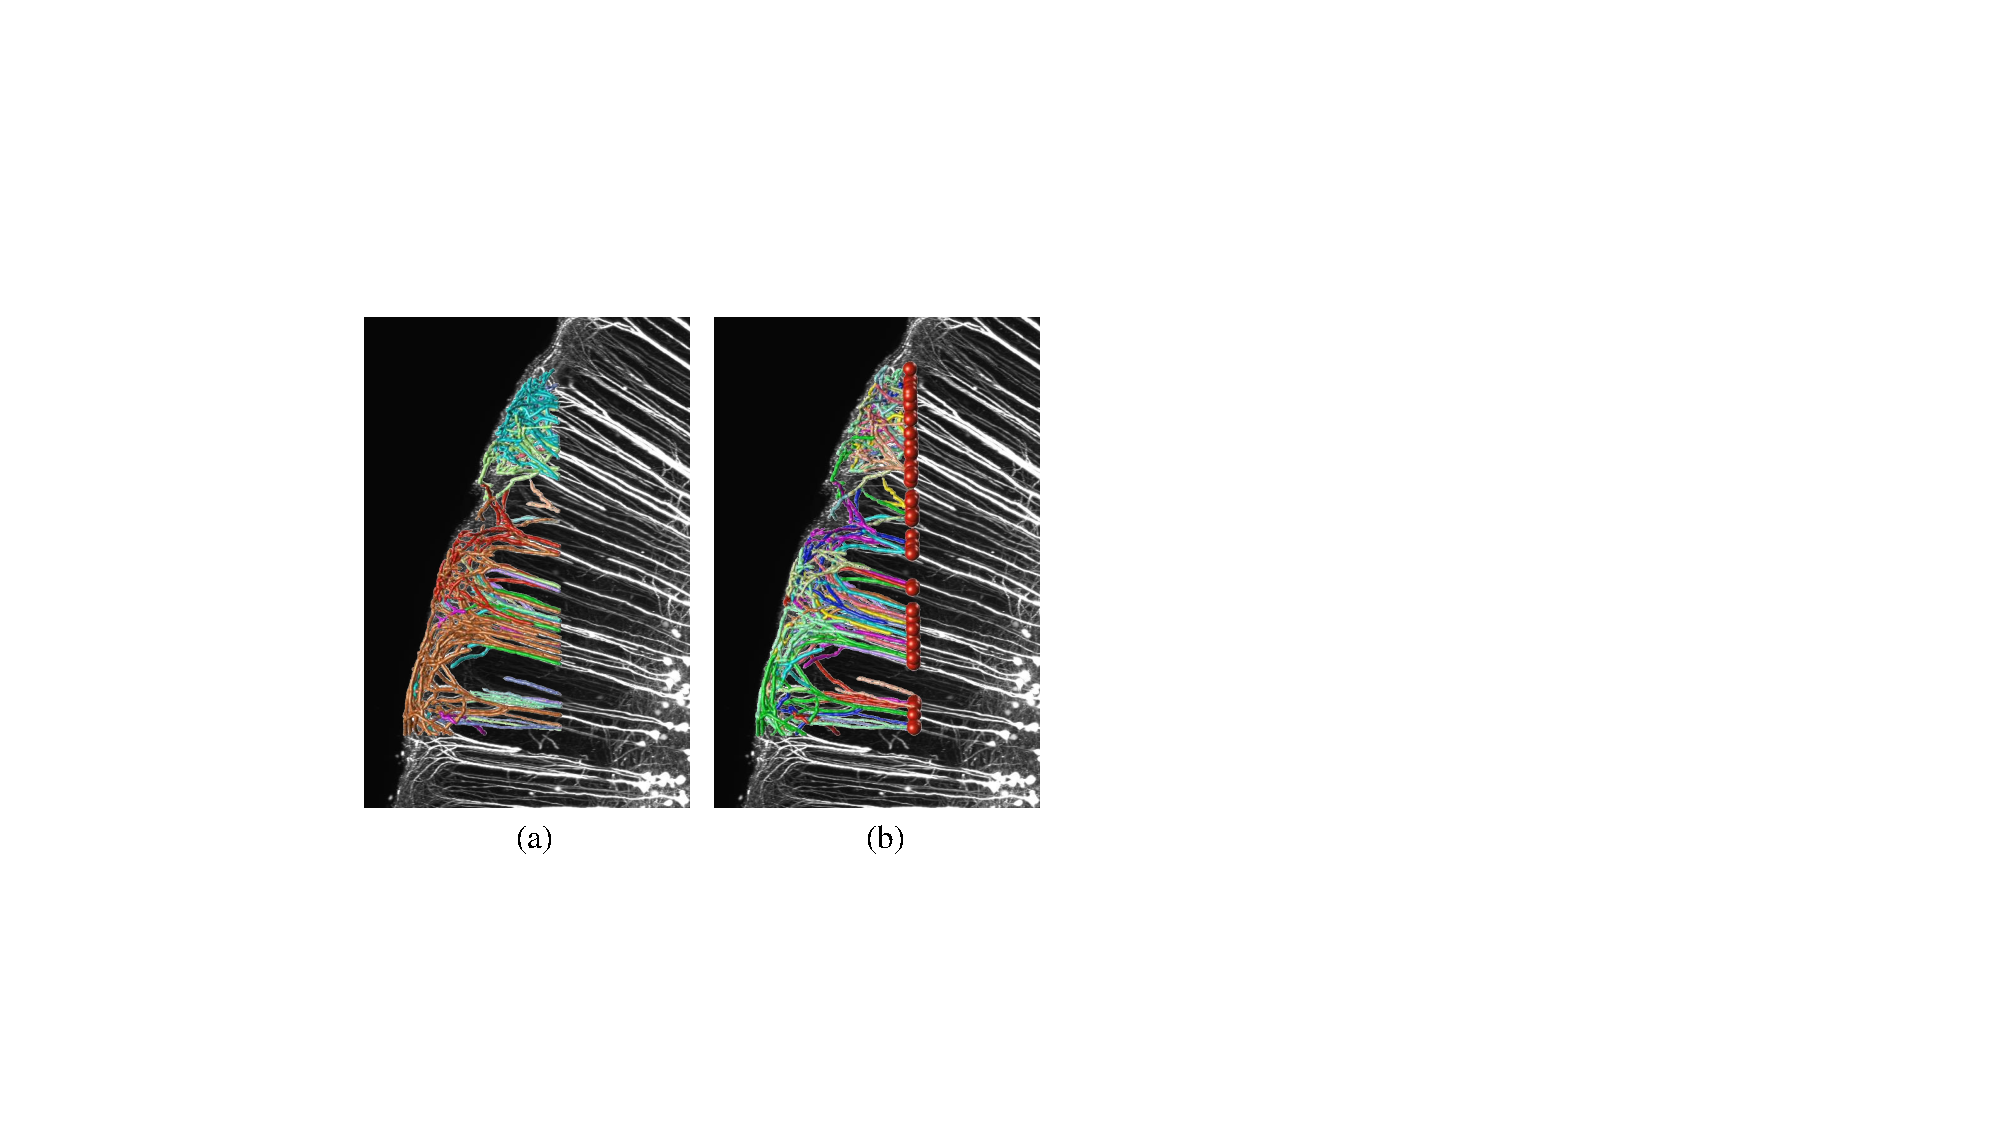
\includegraphics[width=0.85\columnwidth]{./Illustrations/ngpst_pseudosoma.pdf}
	\caption{Comparison of neuron reconstruction results from an enhanced image block by NGPST without setting somas (a) and setting neurite tips (red points) from a neighboring block as pseudo somas (b). Separated neurons are shown in different colors.}
	\label{fig:ngpst_pseudosoma}
\end{figure}



\subsubsection{Neurite Fusion in Adjacent Blocks}
\label{sec:fusion}


\begin{figure}[t]
	\centering
	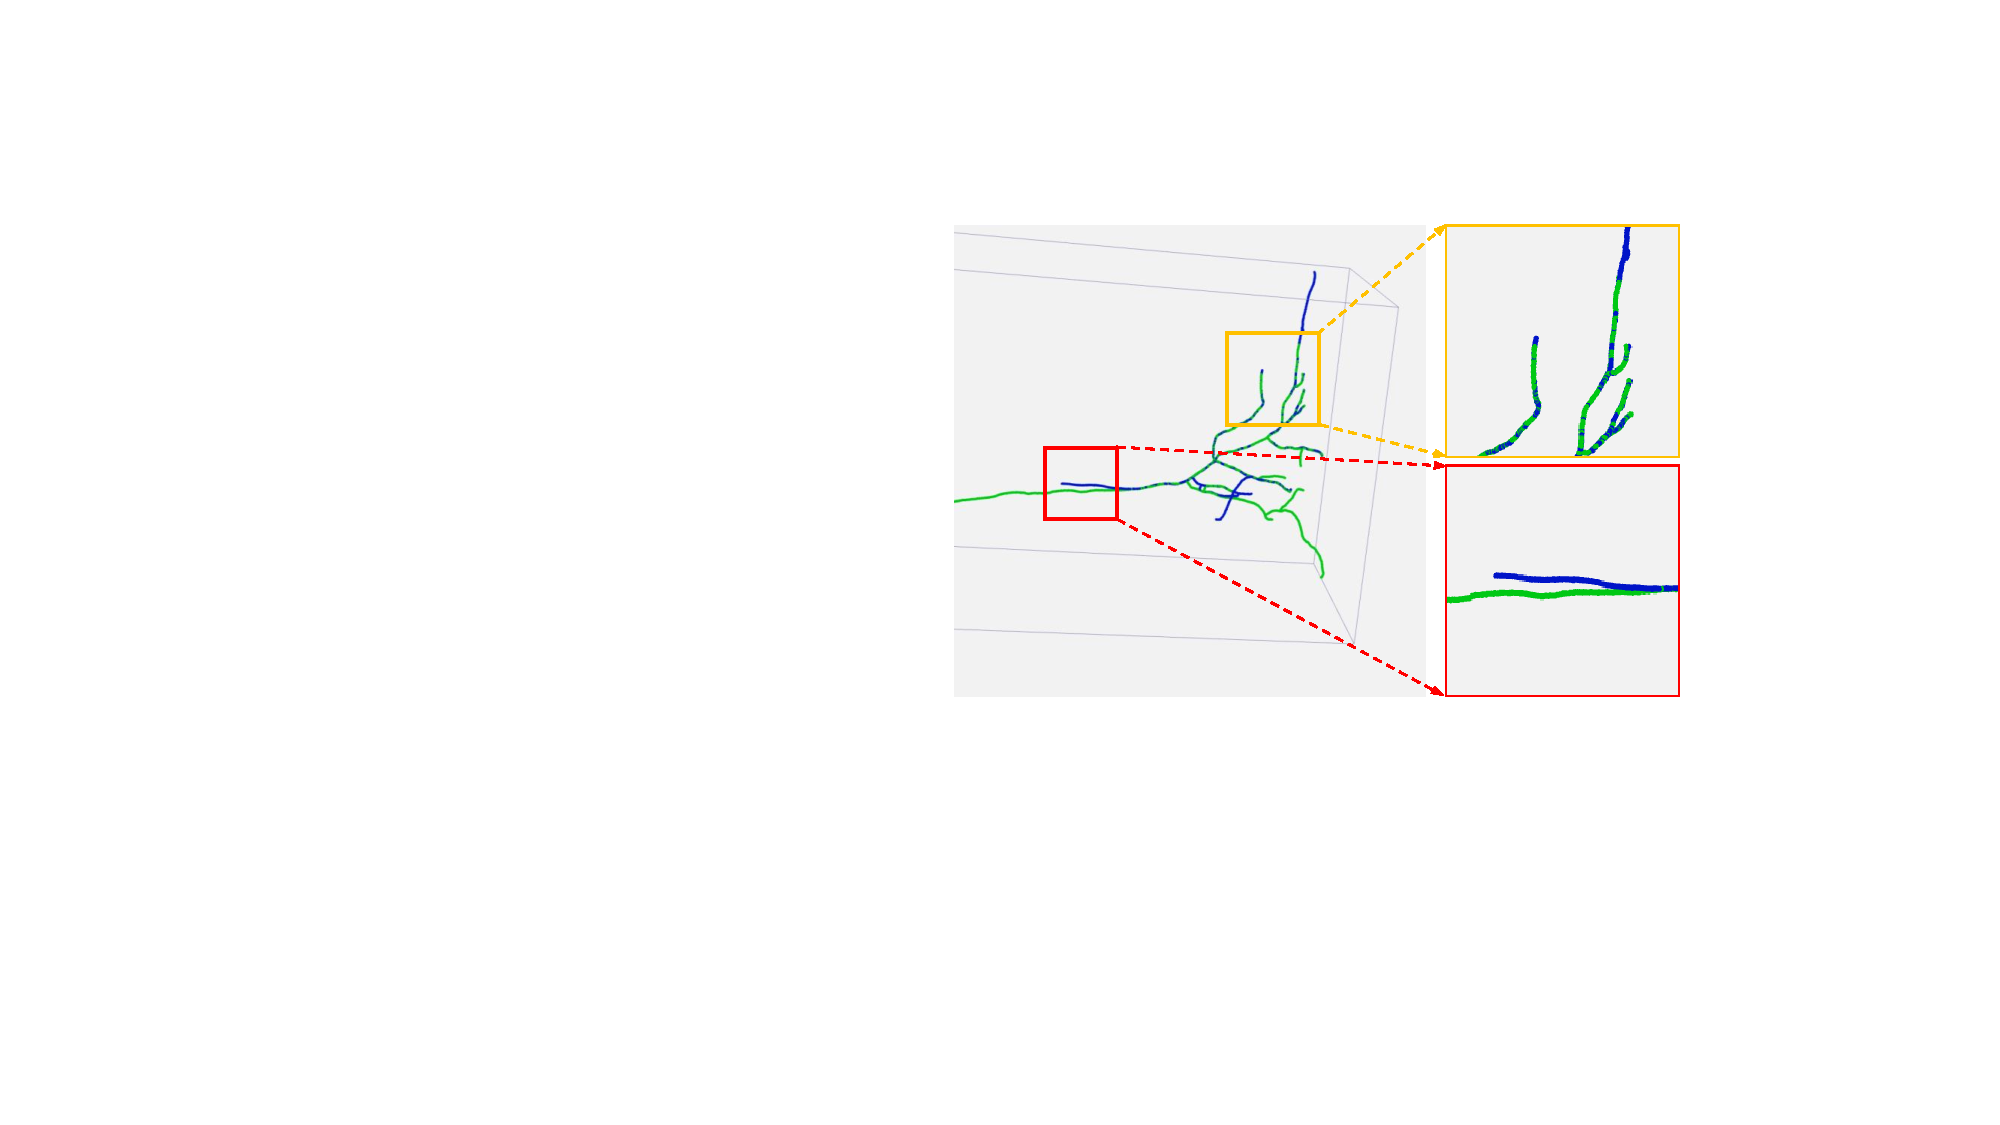
\includegraphics[width=0.86\columnwidth]{./Illustrations/fusion_errors.pdf}
	\caption{An example of over-tracing (yellow) and topological discrepancy (red) when assembling two overlapped neurites. These reconstructions are shown in skeleton mode for better visualization.}
	\label{fig:overlap_discrepancy}
\end{figure}
Since neurons would be split into fragmented neurites when dividing the raw image into blocks, we now fuse the neurites reconstructed separately from adjacent blocks into individual and complete neurons.
Given the reconstructed neurite sets $\mathcal{N}_a$ and $\mathcal{N}_b$ in two overlapped blocks $\mathbf{B}_a$ and $\mathbf{B}_b$ respectively, for any pair of neurites $N_a$ and $N_b$ in the two sets respectively, if their overlapping volume is larger than a threshold $\delta_{ovlp}$, we fuse them together to get a more complete neurite.

There might be over-tracing and topological discrepancy between two neurites that are reconstructed in two blocks separately, as shown in Fig.~\ref{fig:overlap_discrepancy}.
Generally, the reconstruction quality near the block boundary is less accurate and reliable than that in the middle of blocks because of less context. 
Therefore, when fusing two neurites, we tend to keep the neurite segments in the middle of blocks as following.
%But this region is inside the adjacent block due to the overlap between them, which means substantial context information of this region can be provided to the tracing methods and leads to a better reconstruction.
%Therefore, when assembling two matched neurites from adjacent blocks, we only consider neuronal \md{points} which are not near the boundary of the corresponding block. 
  
To fuse two neurites, we first select the longer one as the reference neurite $N_a$, and fuse the other neurite $N_b$ to the reference neurite, as shown in Fig.~\ref{fig:fusion_algorithm} (b).
%
Each neurite is decomposed to a set of neurite branches, as Fig.~\ref{fig:fusion_algorithm} (c) shows.
Each branch is sampled uniformly into a set of neuron compartments, as Fig.~\ref{fig:fusion_algorithm} (d) shows.
%
For each branch $\brc_b$ of neurite $N_b$, we search the branch $\brc_a$ of $N_a$ which has the largest overlapped volume with $\brc_b$, as Fig~\ref{fig:fusion_algorithm} (f) shows.

To fuse the matched two branches, for each point $p_a$ in the branch $\brc_a$, if $p_a$ lies in the boundary region of block $\blk_a$ ($\delta_{bound}$ voxels to the block boundary of $\blk_a$), it will be removed and all its child branches are also deleted, as shown in Fig~\ref{fig:fusion_algorithm} (g).  
The same deletion operation is performed on the points in the branch $\brc_b$ that are located in the boundary regions of block $\blk_b$.
%
Then, for each remaining point $p_b$ in branch $\brc_b$, if there is a point $p_a$ in branch $\brc_a$ so that $dis(p_b,p_a)<\delta_{pt}$, it will be removed since the point $p_a$ is kept, as Fig~\ref{fig:fusion_algorithm} (g) shows.
%
After that, the remaining part of branch $\brc_b$ is merged to the reference branch $\brc_a$ by connecting it to the nearest point in $\brc_a$.
After all matched branches are processed as above, we can obtain the fused neurite $N_{ab}$.
%
For the remaining branches in $N_b$ which are not fused to any branches in $N_a$, they will be merged to the neurite $N_{ab}$ by connecting each of them to the nearest point in $N_{ab}$.
%
Fig~\ref{fig:fusion_algorithm} (h) shows the final fusion result of the two neurites. 
By fusing all neurites in two adjacent blocks, we can obtain more complete reconstruction of dense neuronal populations, as shown in Fig~\ref{fig:fusion_algorithm} (e).


 
 \begin{figure}[t]
 	\centering
 	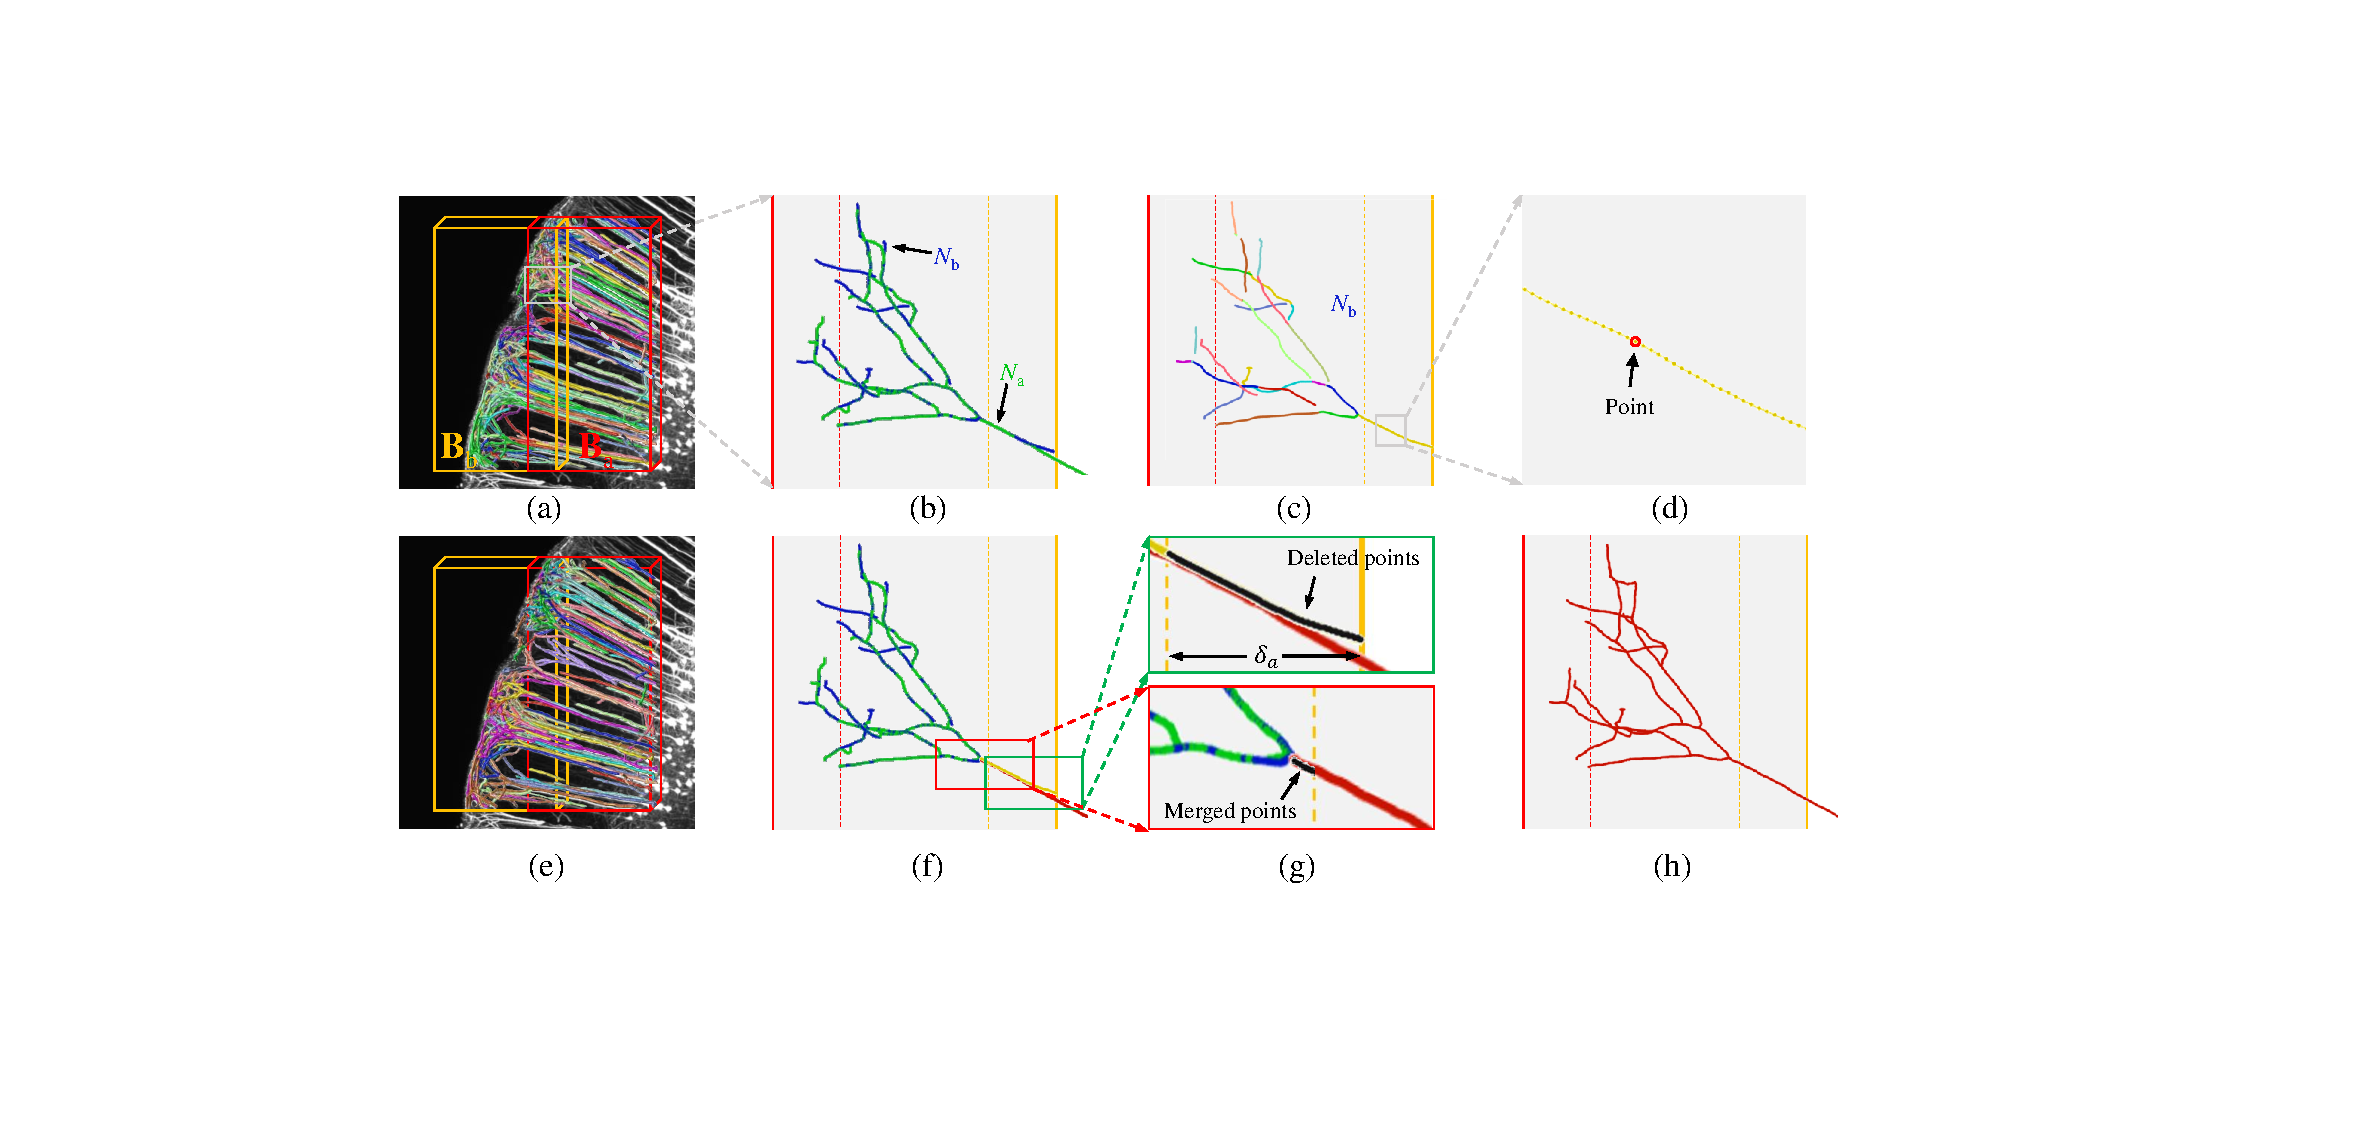
\includegraphics[width=1\columnwidth]{./Illustrations/fusion_algorithm.pdf}
 	\caption{Neurite fusion in two adjacent blocks. (a) Neurites reconstructed separately in two blocks. For two matched neurites $N_a$ and $N_b$ (b), each neurite is decomposed to branches (c) and each branch is sampled into points (d). We delete the points in the boundary regions and merge the points in the middle area of the block (g) to get a more smooth and complete neurite (h). (e) Fusion results of two blocks. }
 	\label{fig:fusion_algorithm}
 \end{figure}
 
 



\section{Experiments and Results}
\label{sec:experiments}

We evaluate our neuron population reconstruction approach in an ultra-scale OM image slice of a mouse brain in dimension of $25397\times 18516\times 869$ ($761$ GB), as Fig.~\ref{fig:brain} shows.
%
The image was captured by the VISoR imaging system~\cite{Wang2019} at a physical resolution of $0.5 \times0.5 \times 0.5$ \SI{}{\micro\metre}$^3$ per voxel. 
%
The image intensity is in 16-bit dynamic range, which preserves sufficient signal details.
In order to evaluate our PLNPR method for neuronal reconstruction in local blocks, we first conduct extensive experiments on the VISoR-40 dataset which we build and the BigNeuron dataset~\cite{peng2015}. 
%
Then we test our UltraNPR algorithm for neuronal population reconstruction in a slice of the mouse brain image.

\subsection{Evaluation of PLNPR on VISoR-40 Dataset}
\label{sec:exp_PLNPR_VISoR}

\subsubsection{VISoR-40 Dataset}
Though many neuron tracing techniques have been proposed, no dataset of OM images has been built for dense neuronal population reconstruction.
We construct a neuron image dataset ``VISoR-40'' (available at \url{https://braindata.bitahub.com/Neuronal_population_reconstruction.html}) for evaluation. 
The VISoR-40 dataset consists of 40 OM image blocks cropped from the mouse brain image. The dimension of the blocks ranges from $419 \times1197 \times 224$ to $869 \times1853 \times 575$.
%
We randomly select $32$ blocks for progressively training the segmentation network without manual annotation in our PLNPR.
%
The remaining 8 blocks with manual annotations are used as the test data.
Each image block for test was first labeled manually and independently by two experts. Then, by cross-checking their results, their agreed annotations were approved by another expert to generate the final ground truth.

\subsubsection{Experimental Settings and Evaluation Metrics}


Pytorch is adopted to implement the DSN model. At each iteration of the progressive learning, the network is trained from scratch with weights initialized from a Gaussian distribution with zero-mean and variance of $ 0.01 $. The optimization is realized with the stochastic gradient descent algorithm with the Adam update rule (batch size of 1, weight decay of $ 0.0005 $, momentum of $ 0.9 $). The base learning rate is set to $ 0.001 $ and descended with the ``poly" learning rate policy (power of $ 0.9 $ and the maximum iteration number of $ 24000 $). 
%The cube size is set as $160\times 160\times 160$ considering the GPU memory limitation.

To quantitatively evaluate our method, four commonly used metrics defined in \cite{Quan2015}, including precision, recall, F-Score, and Jaccard, are computed to measure the fidelity between the reconstruction results and the ground truth. 
Their definitions are defined as follows:
\begin{flalign}
&Precission(R,G)= \frac{\vert R \cap G\vert}{\vert R\vert} = \frac{\vert TP\vert}{\vert R\vert}, & \\
&Recall(R,G) = \frac{\vert R\cap G\vert}{\vert G\vert} = \frac{\vert TP\vert}{\vert G\vert}, & \\
&F{-}Score(R,G)= \frac{2\vert R \cap G\vert}{\vert R\vert + \vert G\vert} = \frac{2\vert TP\vert}{\vert R\vert + \vert G\vert}, & \\
&Jaccard(R,G)= \frac{\vert R\cap G\vert}{\vert R\cup G\vert} = \frac{\vert TP\vert}{\vert R\cup G\vert}, &
\label{equ: metrics}
\end{flalign}
%
where $R$ denotes the set of points on the reconstructed neurons, $G$ denotes the set of neuron points in the ground truth and $TP$ denotes the set of true positive points, $|\cdot|$ denotes the number of points in a set.
%We follow the rule of determining true positive points described in~\cite{Quan2015}. 
The four metrics are first computed on each individual neuronal tree according to the manually labeled skeleton, and then averaged in a neuronal population weighted by the total length of the neuronal processes of each neuron, the same as \cite{Quan2015}.



\subsubsection{Progressive Learning}

The key idea of PLNPR is to progressively improve the performance of neuron reconstruction by making the neuron segmentation network and the conventional tracing method complementary and synergistic without using any manual annotations.
In order to demonstrate the performance improvement, four widely-used tracing methods, including APP1~\cite{Peng2011}, APP2~\cite{Xiao2013}, MOST~\cite{Wu2014} and NGPST~\cite{Quan2015}, are tested as the neuron tracing module in our framework. 
We use their implementations in the software Vaa3D~\cite{Peng2014}. 
%
Eight iterations are tested on our VISoR-40 dataset, and the improvement of neuronal population reconstruction is shown in Fig.~\ref{fig:ablation_study_plnpr}~(a).
We only show the F-Score which is widely used to reflect the overall performance of neuron reconstruction.
%
Moreover, the neuron reconstruction results on a test block at different iterations are shown in the Fig.~\ref{fig:trace_iterations}.
%
\xj{More qualitative and quantitative results are reported in the supplementary materials.}
The results show that our progressive learning strategy effectively facilitates conventional tracing methods to reconstruct more complete neuronal populations.
In addition, the performance improvement gets stable after five iterations of the progressive learning for all the tested tracing methods. 

 

\begin{figure*}[t]
	\centering
	\subfigure[]{
		\begin{minipage}[b]{0.32\linewidth}
			\centering
			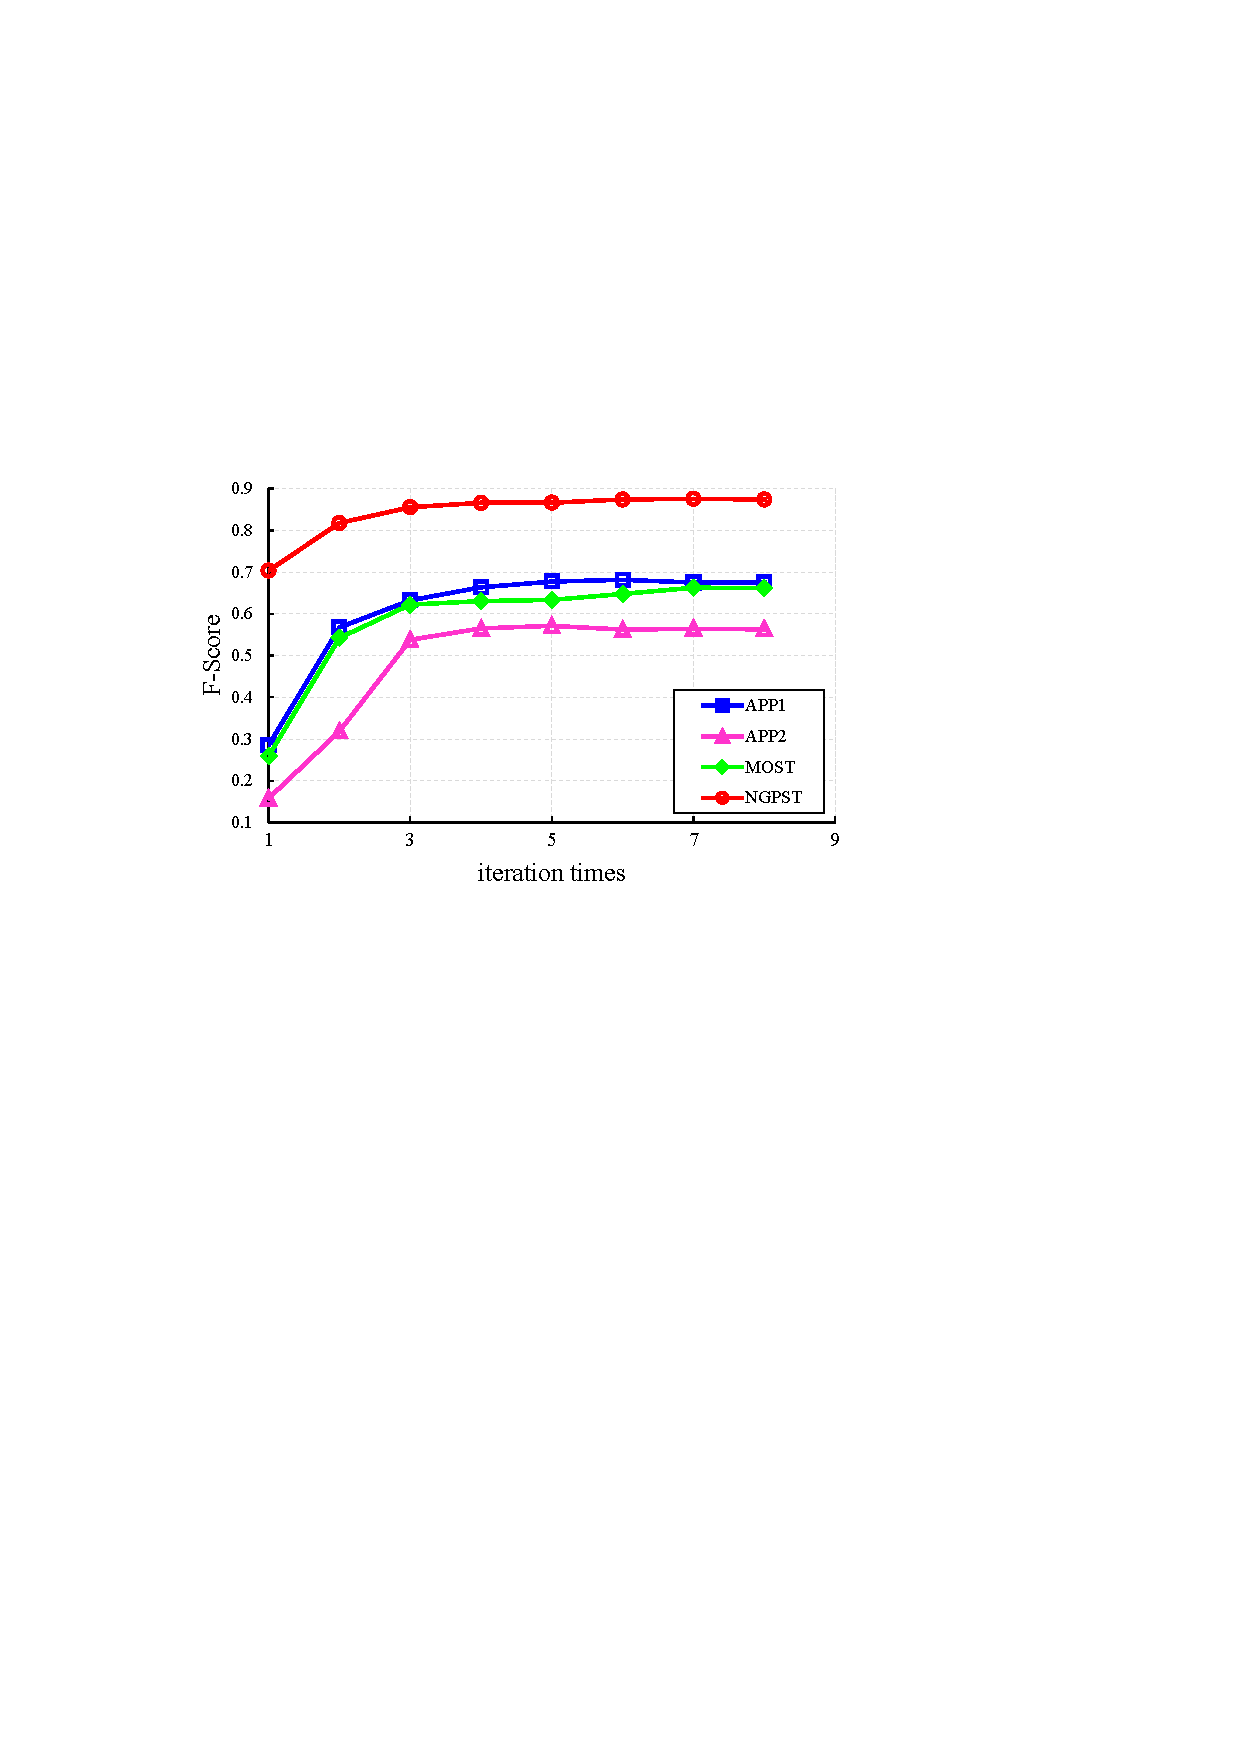
\includegraphics[height=3.7cm]{./Illustrations/trace_iterations_fscore8.pdf}
		\end{minipage}}
	\subfigure[]{
		\begin{minipage}[b]{0.32\linewidth}
			\centering
			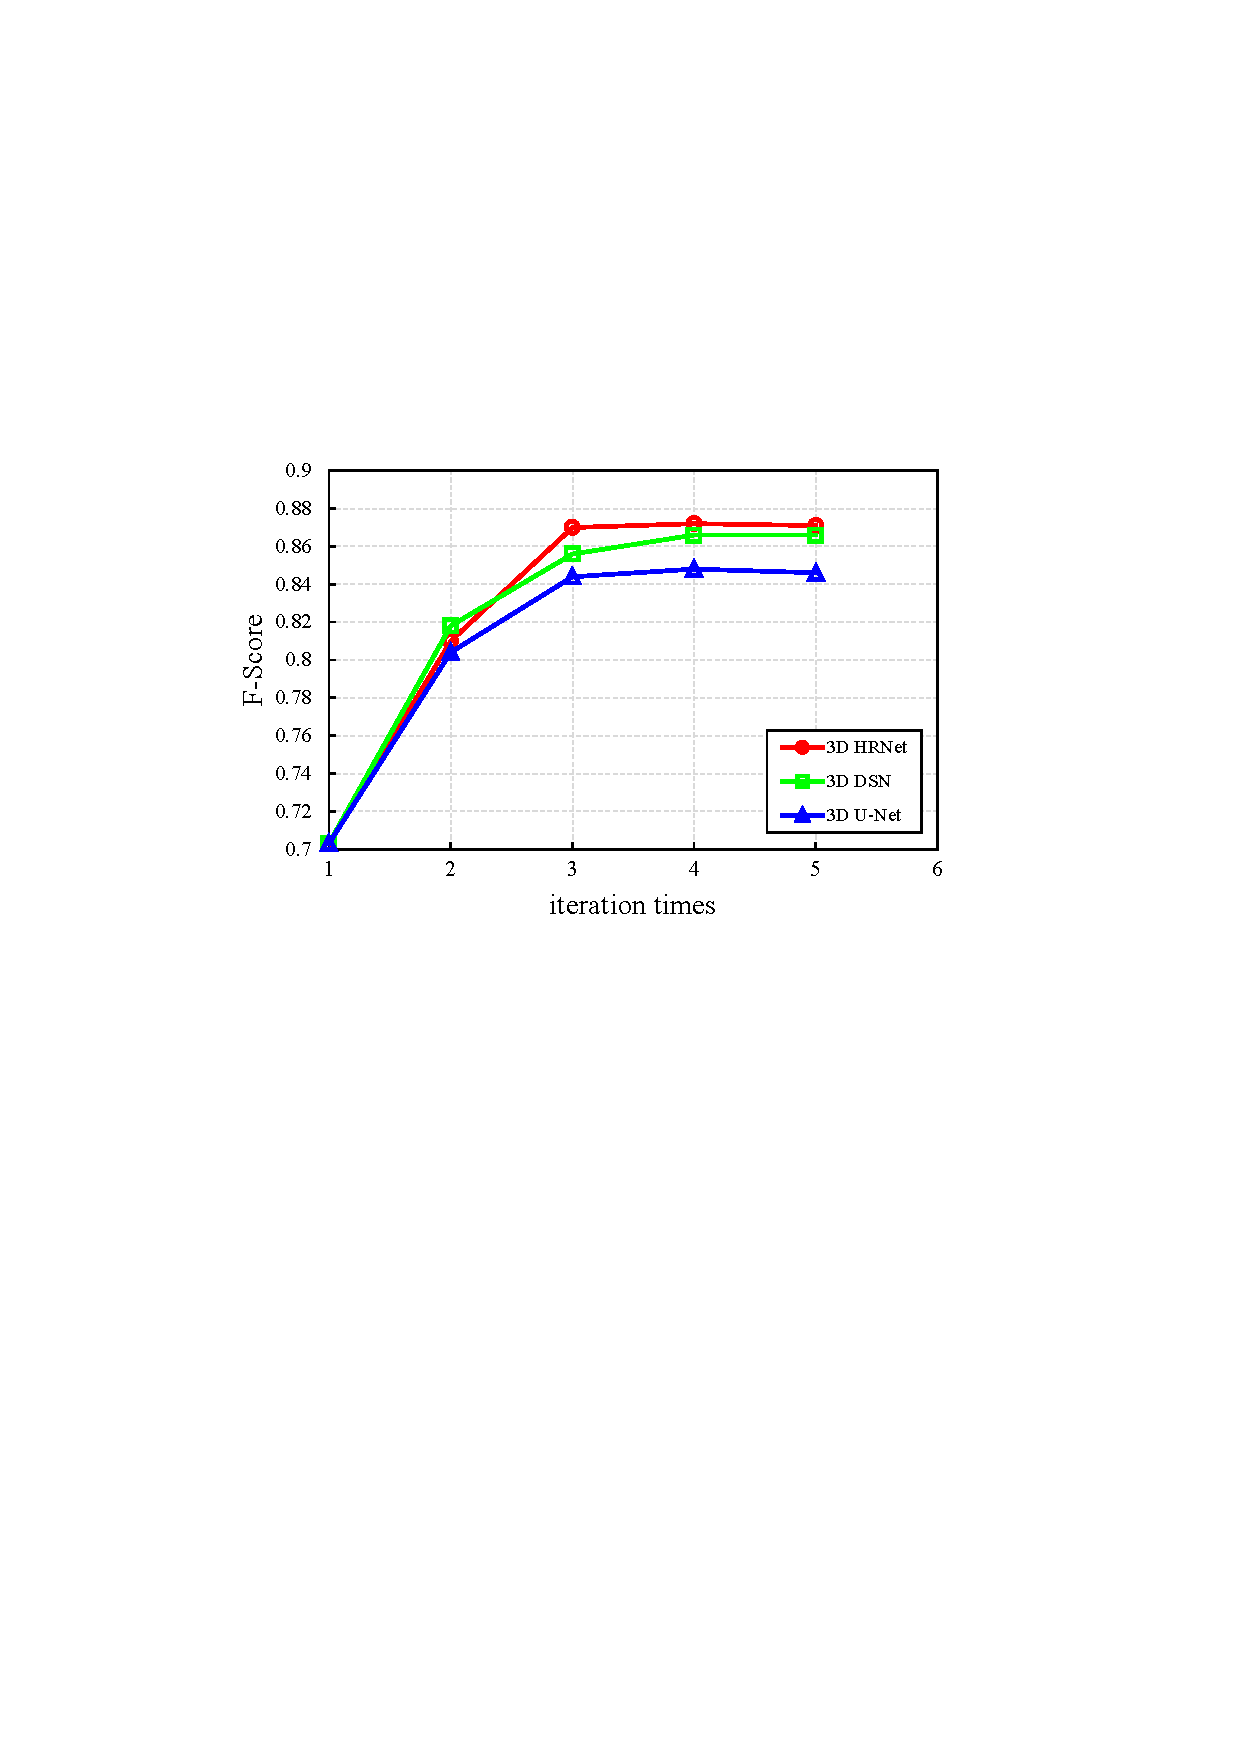
\includegraphics[height=3.7cm]{./Illustrations/trace_networks_fscore11.pdf}
		\end{minipage}}
	\subfigure[]{
		\begin{minipage}[b]{0.32\linewidth}
			\centering
			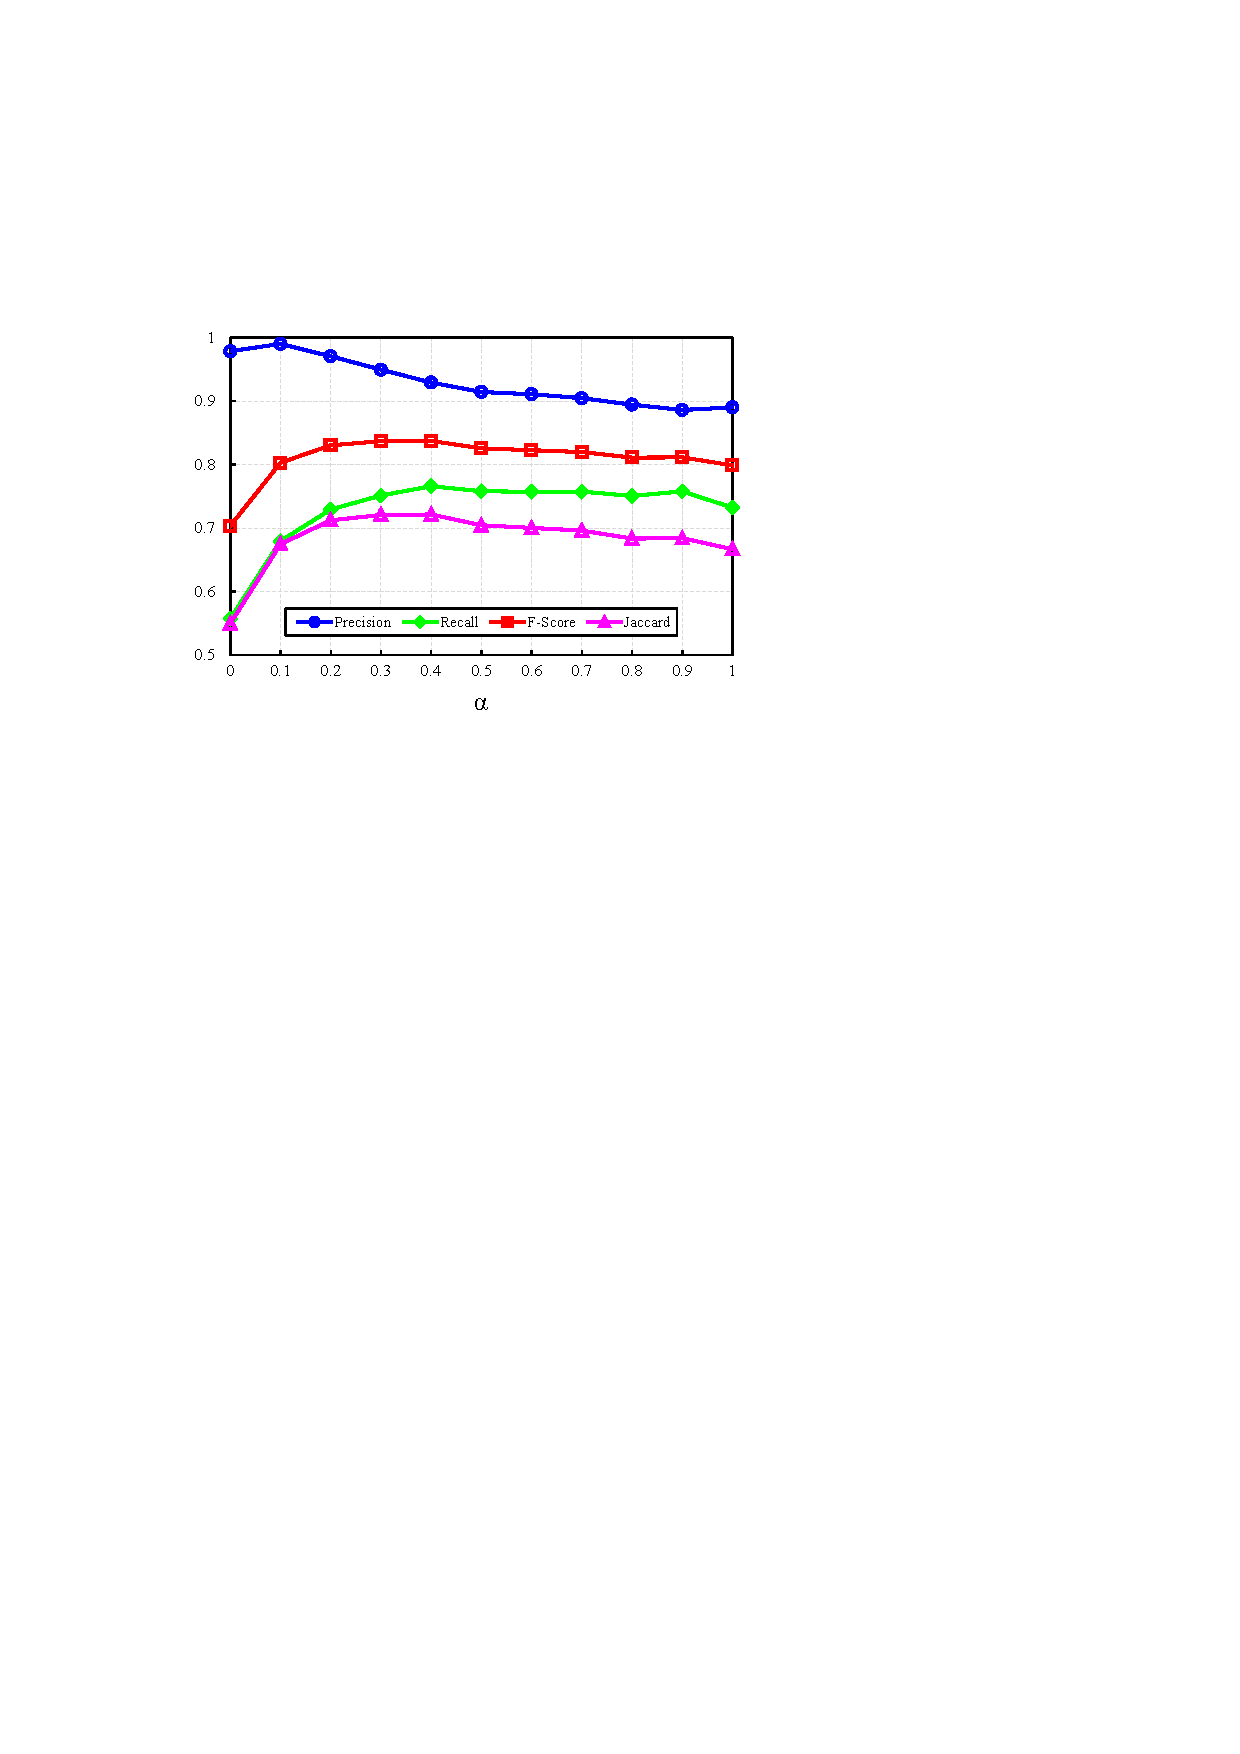
\includegraphics[height=3.7cm]{./Illustrations/weight_paprameter7.pdf}
		\end{minipage}}
	\caption{ Comparison of different parameters in our PLNPR framework on the VISoR-40 dataset.
		(a) Comparisons of neuronal population reconstruction performance at different iterations using four neuron tracing methods. 
		(b) F-Score of neuron reconstruction at five iterations using three deep segmentation networks. 
		Combining any base tracer and any one of the three neuron segmentation networks, our approach progressively improves the reconstruction performance.
		(c) Neuron reconstruction performance with different $\alpha$ in Eq.~\eqref{equ: enhance} for image enhancement.} %From left to right, the value of $\alpha$ increases from $0$ to $1$ by a step of $0.1$.
	
	\label{fig:ablation_study_plnpr}
\end{figure*}


\begin{figure}[t]
	\centering
	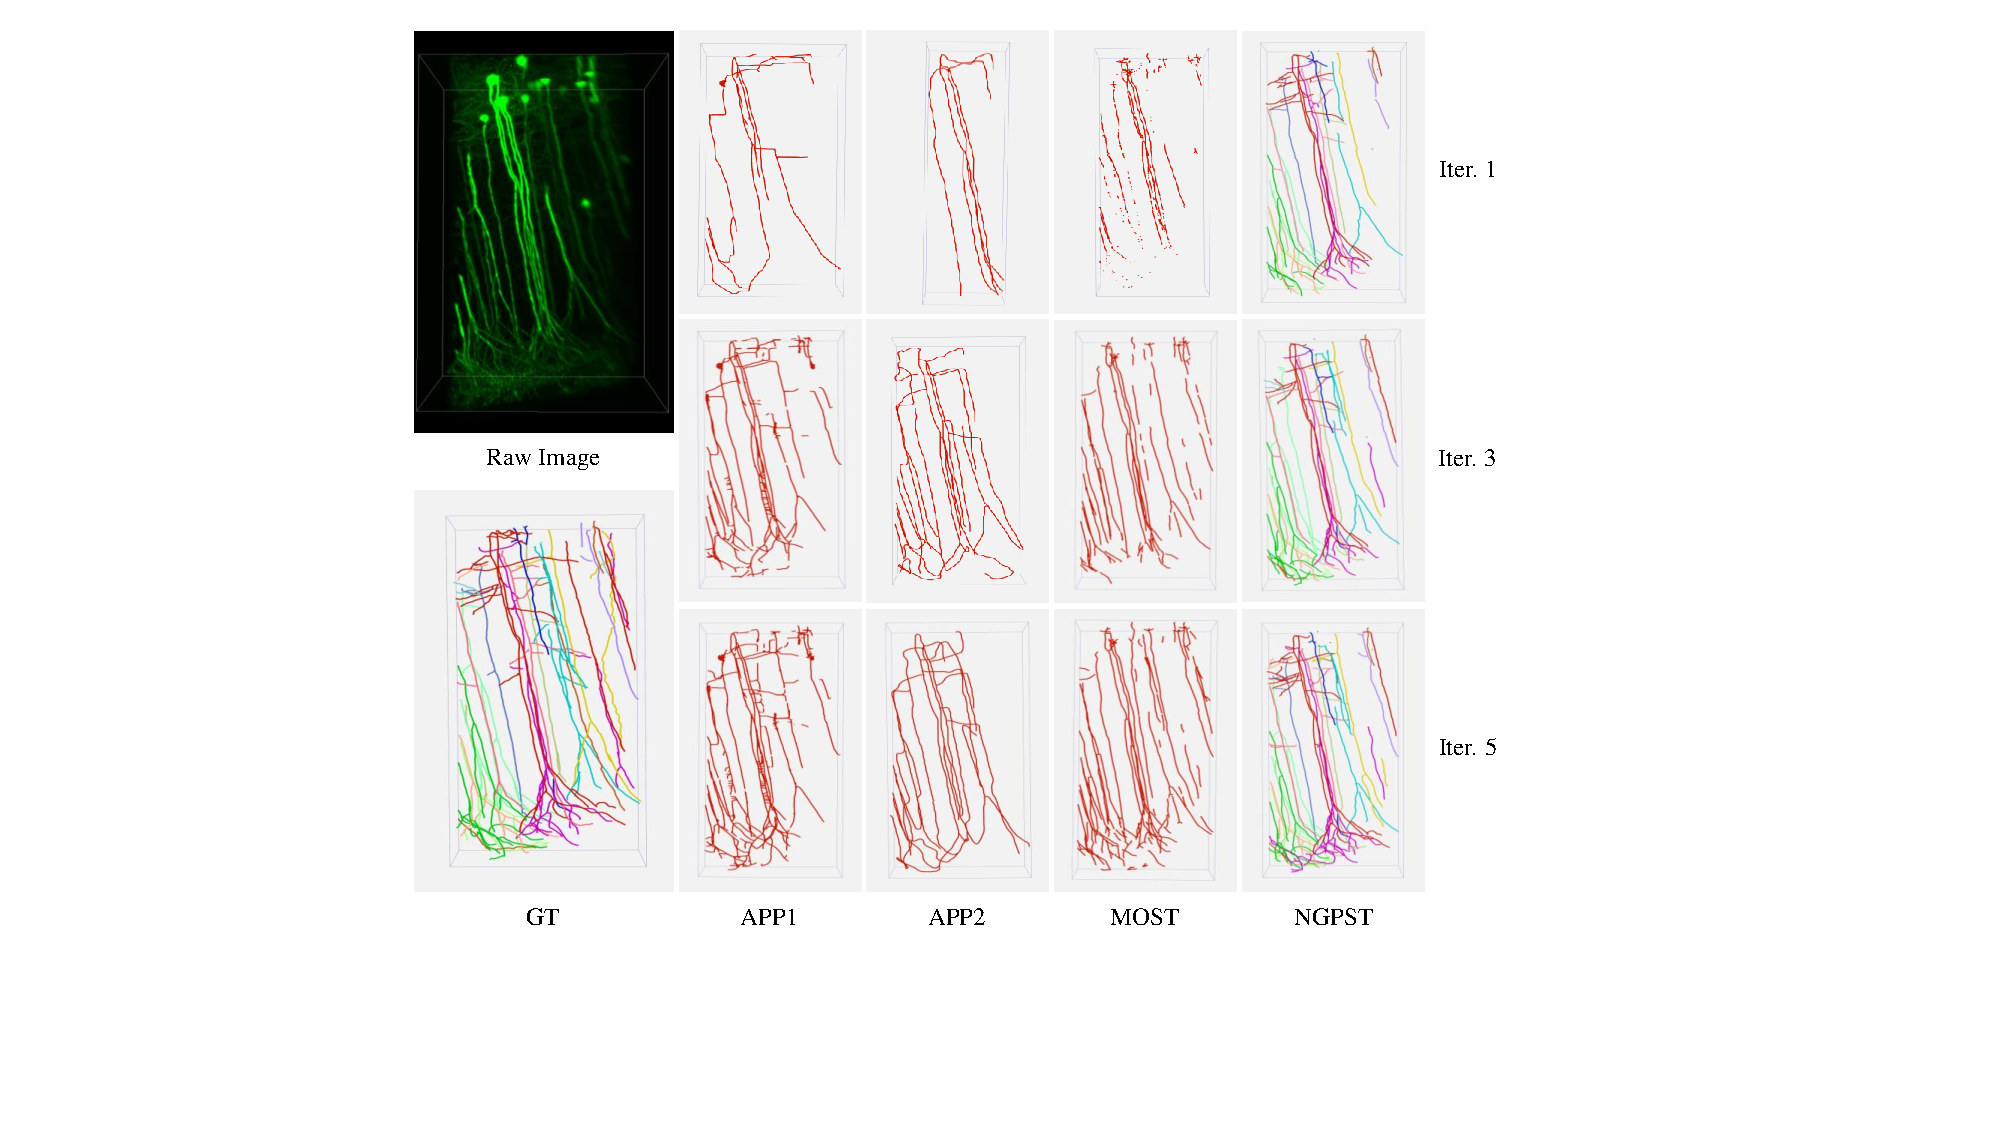
\includegraphics[width=1\columnwidth]{./Illustrations/trace_iterations3.pdf}
	\caption{Neuronal population reconstruction results of a test block at different iterations (top to bottom) using four neuron tracing methods.} 
	% APP1~\cite{Peng2011}, APP2~\cite{Xiao2013}, MOST\cite{Wu2014} and NGPST~\cite{Quan2015}.}
	\label{fig:trace_iterations}
\end{figure}

\delete{
\begin{figure}[t]
	\centering
	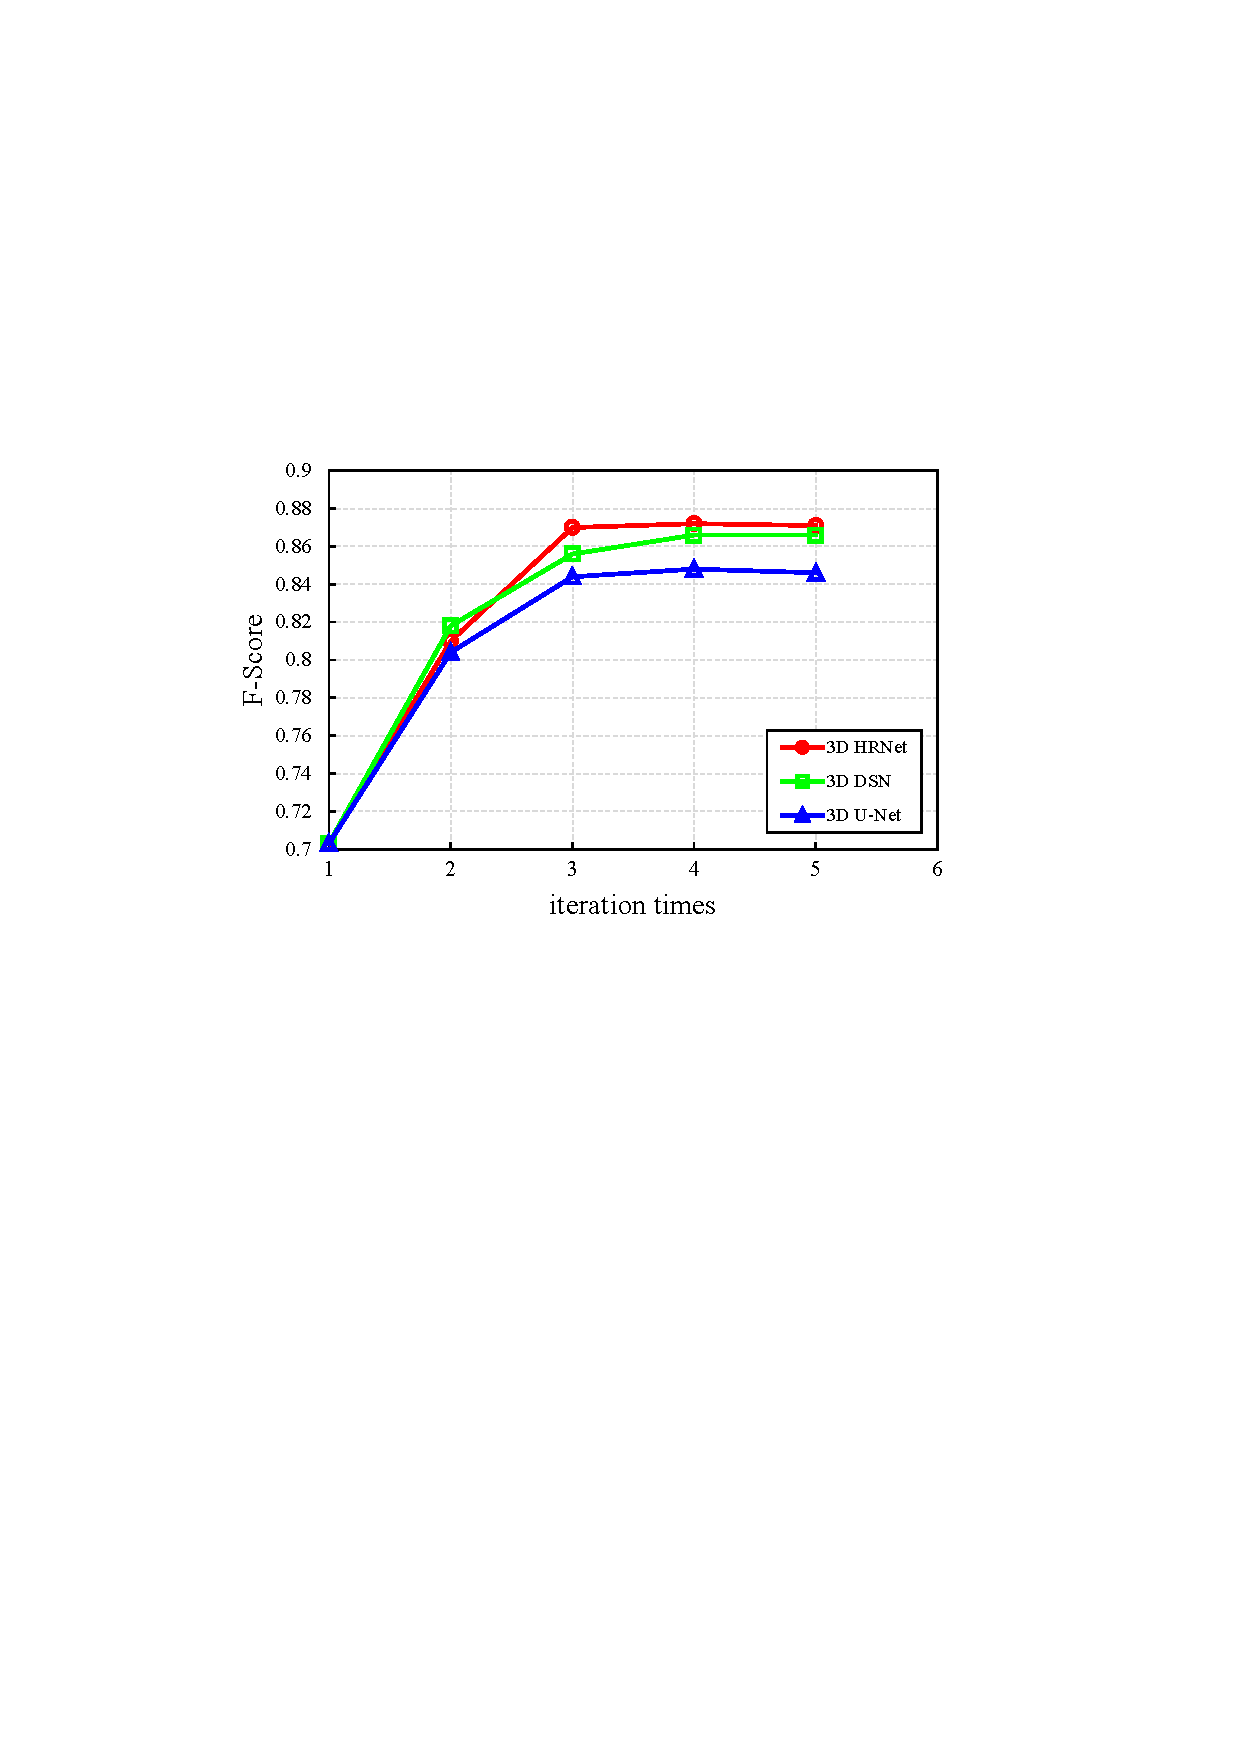
\includegraphics[width=0.8\columnwidth]{./Illustrations/trace_networks_fscore11.pdf}
	\caption{F-Score of neuron reconstruction on the VISoR-40 testing dataset at five iterations. Combining any one of the three neuron segmentation networks, our approach progressively improves the reconstruction performance.}
	\label{fig:fscore_DNNs}
\end{figure}
}


\subsubsection{Neuron Segmentation Network}

To further verify the effectiveness and robustness of our progressive learning strategy, we test three commonly-used deep segmentation networks, including 3D DSN~\cite{Dou2017}, 3D U-Net~\cite{Cicek2016} and a 3D version of HRNet~\cite{Sun2019}, for generating the neuron probability map.
Five iterations are tested on our VISoR-40 dataset, and the F-Score improvement of reconstruction results is shown in Fig.~\ref{fig:ablation_study_plnpr}~(b). 
%
It can be seen that our PLNPR algorithm effectively improves the neuron reconstruction performance by combining any one of the three neuron segmentation networks.
Consequently, the segmentation network and traditional tracing method can complement and promote each other, leading to more complete neuron reconstruction.


\subsubsection{Enhancement Parameter} 

In order to explore the influence of parameter $\alpha$ in Eq.~\eqref{equ: enhance} for image enhancement, we adopt different values for $\alpha$, and the results are shown in Fig.~\ref{fig:ablation_study_plnpr}~(c).
$\alpha=0$ means that the raw image block is directly used as input for the tracing module.
$\alpha=1$ means that only the probability maps are used as input for neuron tracing. 
It indicates that the performance is improved by combing the probability map with the raw image signal, mainly because that the probability map reflects the long-range trajectory structures while the original image signal carries more details of subtle neurites.
%Second, it can be observed our system is very robust to the parameter $\alpha$. 
%Hence, the chosen of the parameter $\alpha$ is not very demanding and the reconstruction performance can achieve significant improvement with any $\alpha >0$. 
In this paper, we empirically select $\alpha=0.1$ to reduce the influence of false positive predictions in probability maps due to the limited performance of the DNN model trained by pseudo labels and increase the robustness of the whole framework.

\delete{
\begin{figure}[t]
	\centering
	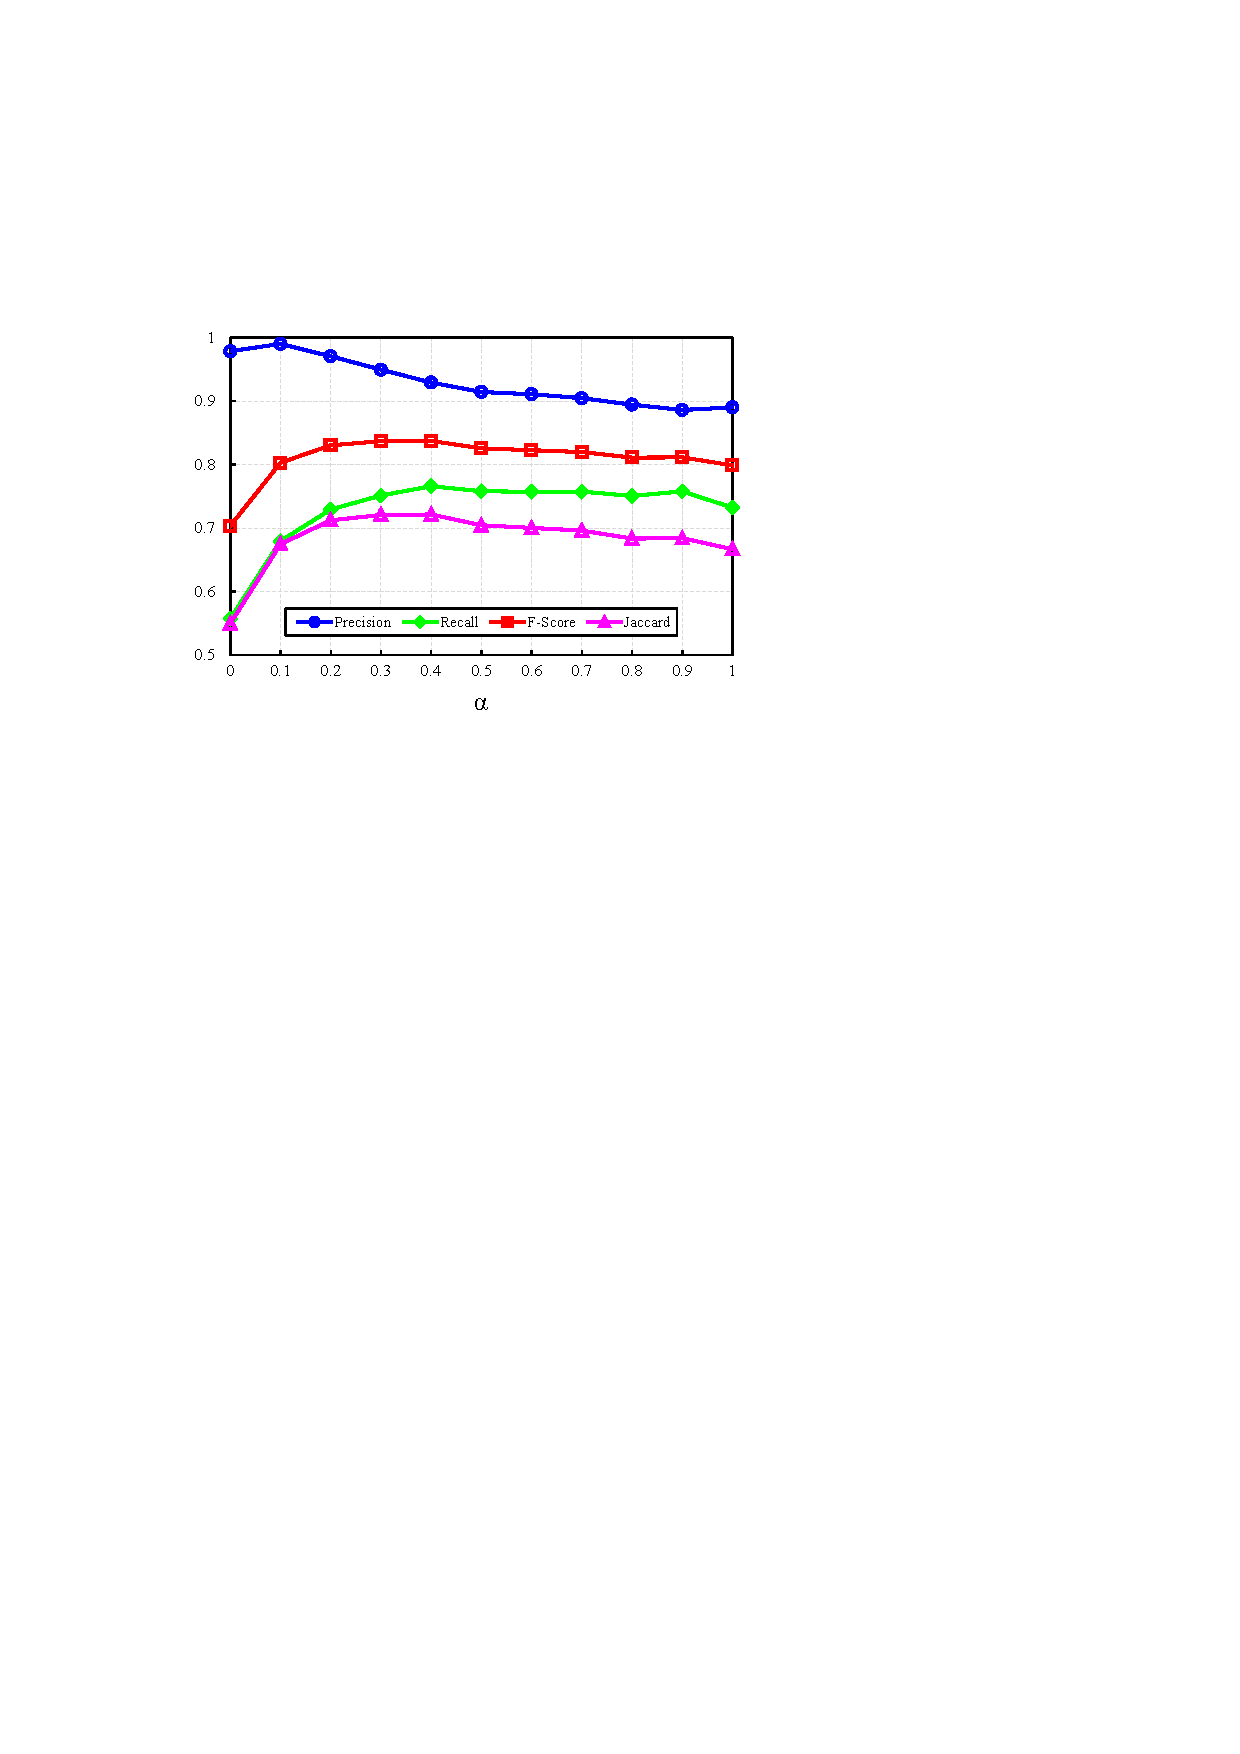
\includegraphics[width=0.8\columnwidth]{./Illustrations/weight_paprameter7.pdf}
	\caption{Neuron reconstruction performance with different $\alpha$ in Eq.~\eqref{equ: enhance} for image enhancement on the VISoR-40 test dataset. From left to right, the value of $\alpha$ increases from $0$ to $1$ by a step of $0.1$.  }
	\label{fig:weight_paprameter}
\end{figure}
}


\subsubsection{Comparison with Tracing Methods}



\begin{figure*}[t]
	\centering
	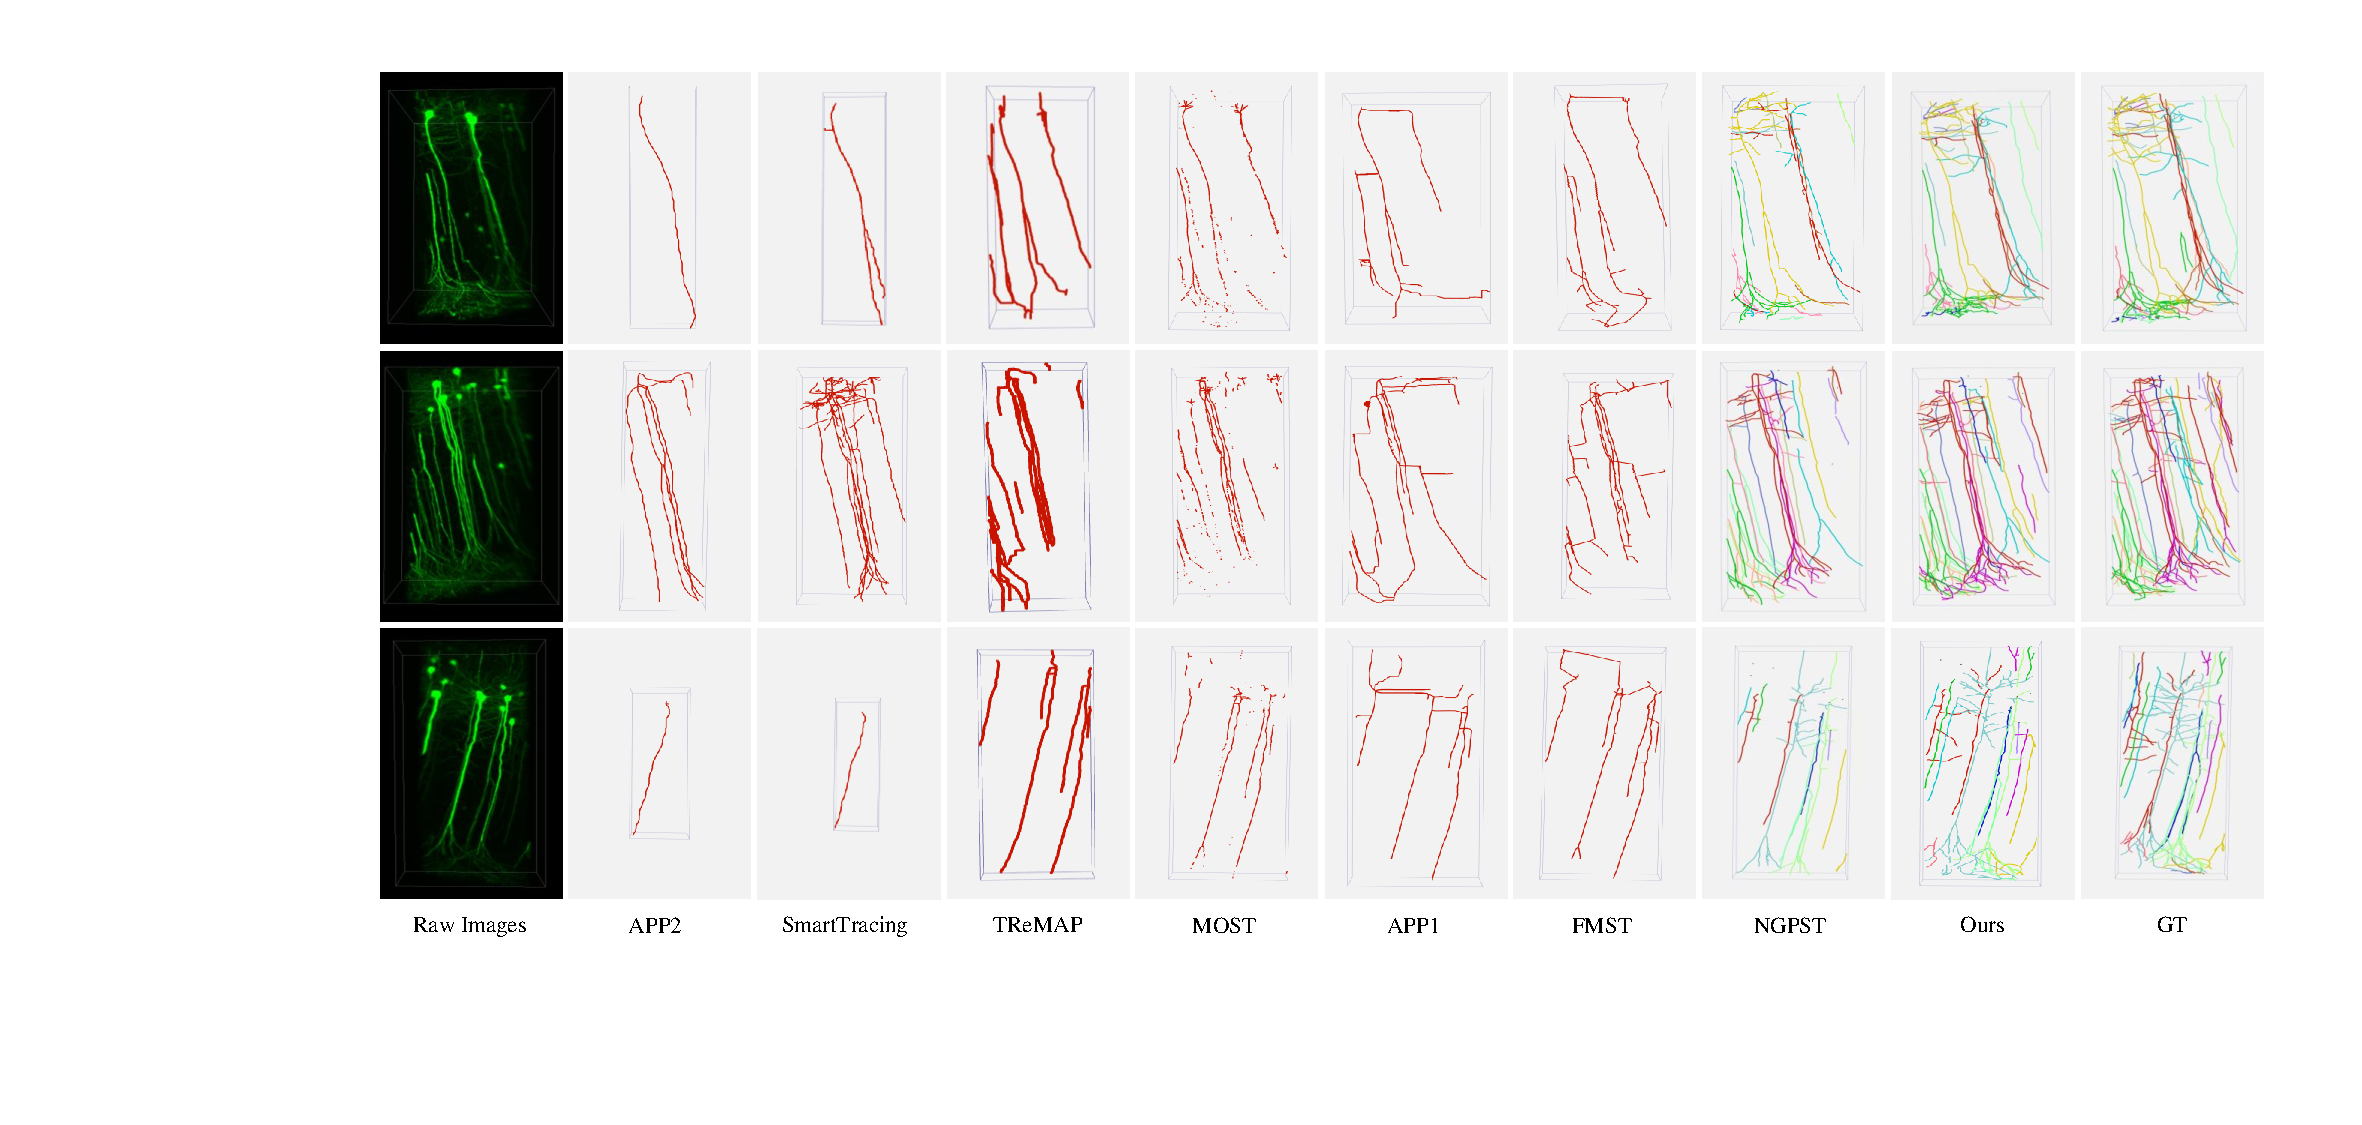
\includegraphics[width=1\textwidth]{./Illustrations/iteration3.pdf}
	\caption{Comparison of neuronal population reconstruction results of three image blocks. %using neuron reconstruction methods FMST~\cite{Yang2019}, APP1~\cite{Peng2011}, APP2~\cite{Xiao2013}, SmartTracing~\cite{Chen2015}, MOST~\cite{Wu2014}, NGPST~\cite{Quan2015} and our PLNPR on three test images from the VISoR-40 dataset.
%	Each row shows the reconstruction results generated by different methods for a test image. The first column shows the raw images, while the last column shows the ground truth (GT). Each of the remaining columns shows the reconstruction result using the corresponding tracing method. 
Our PLNPR method reconstructs more complete and accurate neurons compared to other methods. 
	}
	\label{fig:compare_VISoR}
\end{figure*}



\begin{table*}[th]
	\centering
	\caption{Performance comparison with different methods for neuronal population reconstruction on the VISoR-40 dataset.}
	\label{table:compare_VISoR}
	\begin{tabular}{lcccc}
		\toprule
		Method & Precision & Recall & F-Score & Jaccard\\
		\midrule
		%\hline
		APP2~\cite{Xiao2013}
		& \textbf{0.980} & 0.091 & 0.157 & 0.091\\
		SmartTracing~\cite{Chen2015}
		& 0.961 & 0.133 & 0.205 & 0.128\\
		TReMAP~\cite{Zhou2016}
		& 0.917 & 0.147 & 0.253 & 0.145\\
		MOST~\cite{Wu2014}          
		& 0.969 & 0.151& 0.258& 0.151\\
		APP1~\cite{Peng2011}
		& 0.935 & 0.169 & 0.284 & 0.167\\
		FMST~\cite{Yang2019}
		& 0.884 & 0.179 & 0.296 &  0.176\\
		NGPST~\cite{Quan2015}
		& 0.978 & 0.557& 0.703 & 0.549\\
		\midrule
		Ours
		& 0.971 & \textbf{0.801}&\textbf{0.875} & \textbf{0.781}\\
		\bottomrule
	\end{tabular}
\end{table*}

%<18-AAAI-Adaptive Graph Convolutional Neural Networks>
To prove the effectiveness of our method on neuronal population reconstruction, we compare it with seven widely used neuron tracing methods, including APP1~\cite{Peng2011},  APP2~\cite{Xiao2013}, MOST~\cite{Wu2014}, SmartTracing~\cite{Chen2015}, NGPST~\cite{Quan2015}, TReMAP~\cite{Zhou2016} and  FMST~\cite{Yang2019}.
The parameters of these tracing methods are manually adjusted for each image block to get the optimal performance in our experiments.
%
We utilize NGPST with 3D DSN enhancement as ``Ours''. Note that the segmentation network in our approach is trained progressively on the VISoR-40 dataset in the training stage. We use the trained model directly at the test stage for evaluation. 
%
Table~\ref{table:compare_VISoR} compares the quantitative results of different methods with regard to the four metrics including precision, recall, F-Score, and Jaccard.
%
It shows that our method makes a significant improvement on the overall performance compared with other methods.
Though APP2 achieves the highest precision, the reconstructed neurons are significantly sparser than others. 
%
Fig.~\ref{fig:compare_VISoR} shows the neuronal populations reconstructed from three test image blocks.
Compared with other methods, our PLNPR is superior in both sparse and dense neurons.
Conventional tracing methods~\cite{Peng2011, Xiao2013, Wu2014, Zhou2016} and learning-based methods~\cite{Chen2015, Yang2019} tend to extract the main trunk of neurons, while missing a large portion of subtle neurites. 
Therefore, these methods have very high precision but significantly lower recall.
Although NGPST~\cite{Quan2015} achieves better performance of neuronal population reconstruction compared with other single-neuron tracing methods, it still remains difficult to extract subtle neuron voxels for NGPST by using hand-crafted features.
%
In comparison, our method benefits from the progressively trained segmentation network, and reconstructs more complete neurons from challenging blocks, even there exhibit noises, low contrast, and blending of fluorescence in the blocks.


\subsection{Evaluation of PLNPR on BigNeuron Dataset}
\label{sec:exp_PLNPR_BigNeuron}

\subsubsection{BigNeuron Dataset}

To validate our PLNPR method on single neuron reconstruction, we employ the BigNeuron~\cite{peng2015} dataset.
% which is a well-known community-derived neuron dataset. 
This dataset consists of about $20,000$ 3D OM images in total, acquired from a variety of species and optical imaging systems by different institutes.
%Some images have the corresponding manual annotations for evaluation.  
Unlike our VISoR-40 dataset which is built for the evaluation of neuronal population reconstruction, each block in the BigNeuron dataset only contains a single neuron or fragmented neurites.
% which are appropriate for single neuron reconstruction.
Following \cite{Li2017}, we select the same 68 images that are from a variety of species to evaluate the the performance of dense neurite reconstruction.
Manual reconstruction by experts is associated with each image. 
51 images are used for network training in \cite{Li2017} and the remaining 17 images are used for evaluation.
Note that we do not use the manual annotations in our PLNPR in training the deep neural network. 


\subsubsection{Experimental Settings}
 
 
To evaluate our PLNPR on the single neuron reconstruction, we use the DSN model pretrained on the VISoR-40 dataset as initialization and fine-tune it on the BigNeuron dataset using pseudo labels generated by NGPST~\cite{Quan2015} instead of the provided manual annotations.
%
The learning rate was initialized as $\num{1e-4}$ and decayed using the ``poly" learning rate policy with power of $0.9$. The maximum iteration number is set to $ 24000 $. 
We cropped image patches of size $160\times 160\times 8$ as input to the segmentation network since the axial dimensions are usually much lower in the images of the BigNeuron dataset than our VISoR-40 dataset.
Data augmentation by transposing the three dimensions of each training image is also performed. 


\subsubsection{Comparison on BigNeuron Dataset}

\begin{figure*}[th]
	\centering
	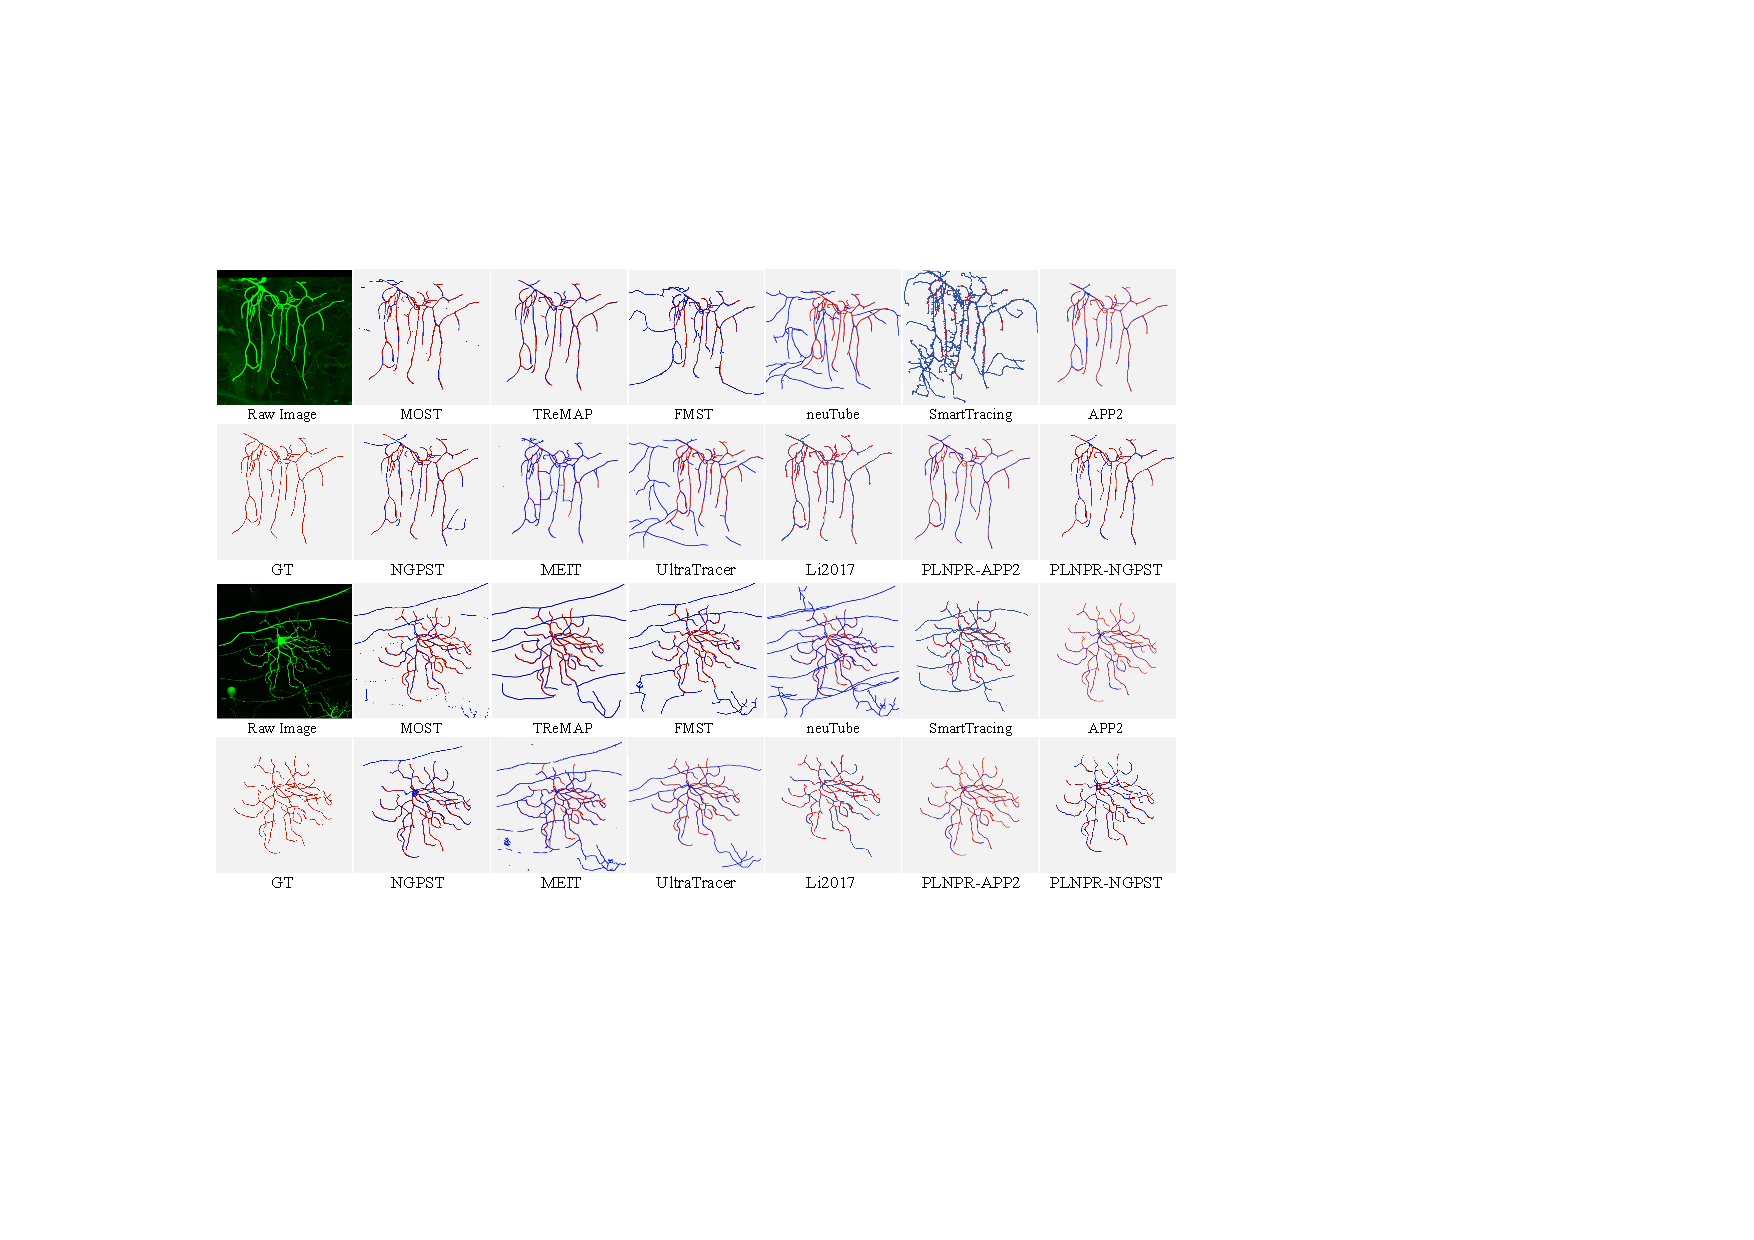
\includegraphics[width=1\textwidth]{./Illustrations/BigNeuron_comparison.pdf}
	\caption{Comparison of single neuron reconstruction results on two test images from the BigNeuron dataset.
		% using MOST~\cite{Wu2014}, FMST~\cite{Yang2019}, APP2~\cite{Xiao2013}, TReMAP~\cite{Zhou2016}, NGPST~\cite{Quan2015}, SmartTracing~\cite{Chen2015}, Li2017~\cite{Li2017} and our PLNPR on two testing images from the BigNeuron dataset.
	The reconstructed neurites are shown in blue and the corresponding ground truth (GT) are shown in red.
	Our method reconstructs more complete and accurate neurons compared to other methods.
	}
	\label{fig:compare_BigNeuron}
\end{figure*}

\begin{table*}[th]
	\centering
	\makeatletter\def\@captype{table}\makeatother
	\caption{Performance comparison for single neuron reconstruction on the BigNeuron test dataset.}
	\label{table:compare_BigNeuron}
	\begin{tabular}{lccccccc}
		\toprule
		Method & Precision & Recall & F-Score & Jaccard & ESA & DSA & PDS\\
		\midrule
		MOST~\cite{Wu2014} & 0.619 & 0.361 & 0.456 & 0.295 & 31.730 & 38.211 & 0.633\\
		FMST~\cite{Yang2019} & 0.575 & 0.629 & 0.601 & 0.429 & 17.878 & 23.459 & 0.558\\
		APP2~\cite{Xiao2013} & 0.799 & 0.492 & 0.608 & 0.437 & 13.457 & 17.923 & 0.562\\
		TReMAP~\cite{Zhou2016} & 0.771 & 0.415 & 0.539 & 0.369 & 11.269 & 17.941 & 0.539\\
		NGPST~\cite{Quan2015} & 0.710 & 0.680 & 0.695 & 0.532 & 10.168 & 14.880 & 0.587\\
		SmartTracing~\cite{Chen2015} & 0.701 & 0.648 & 0.674 & 0.508 & 8.532 & 11.609 & 0.543\\
		Li2017~\cite{Li2017} & - & - & - & - & 4.917 & \textbf{7.972} &0.461 \\
		UltraTracer~\cite{Peng2017} & \textbf{0.808} & 0.548 & 0.653 & 0.485 & 9.578 & 14.197 & 0.452 \\
		MEIT~\cite{Wang2018} &  &  &  & & 12.068 &16.578 & 0.554 \\
		\midrule
		Ours & 0.790 & \textbf{0.707} & \textbf{0.746}  & \textbf{0.595} & \textbf{4.784} & 8.309 & \textbf{0.451}\\
		\bottomrule
	\end{tabular}
\end{table*}

\begin{figure}[t]
	\centering
	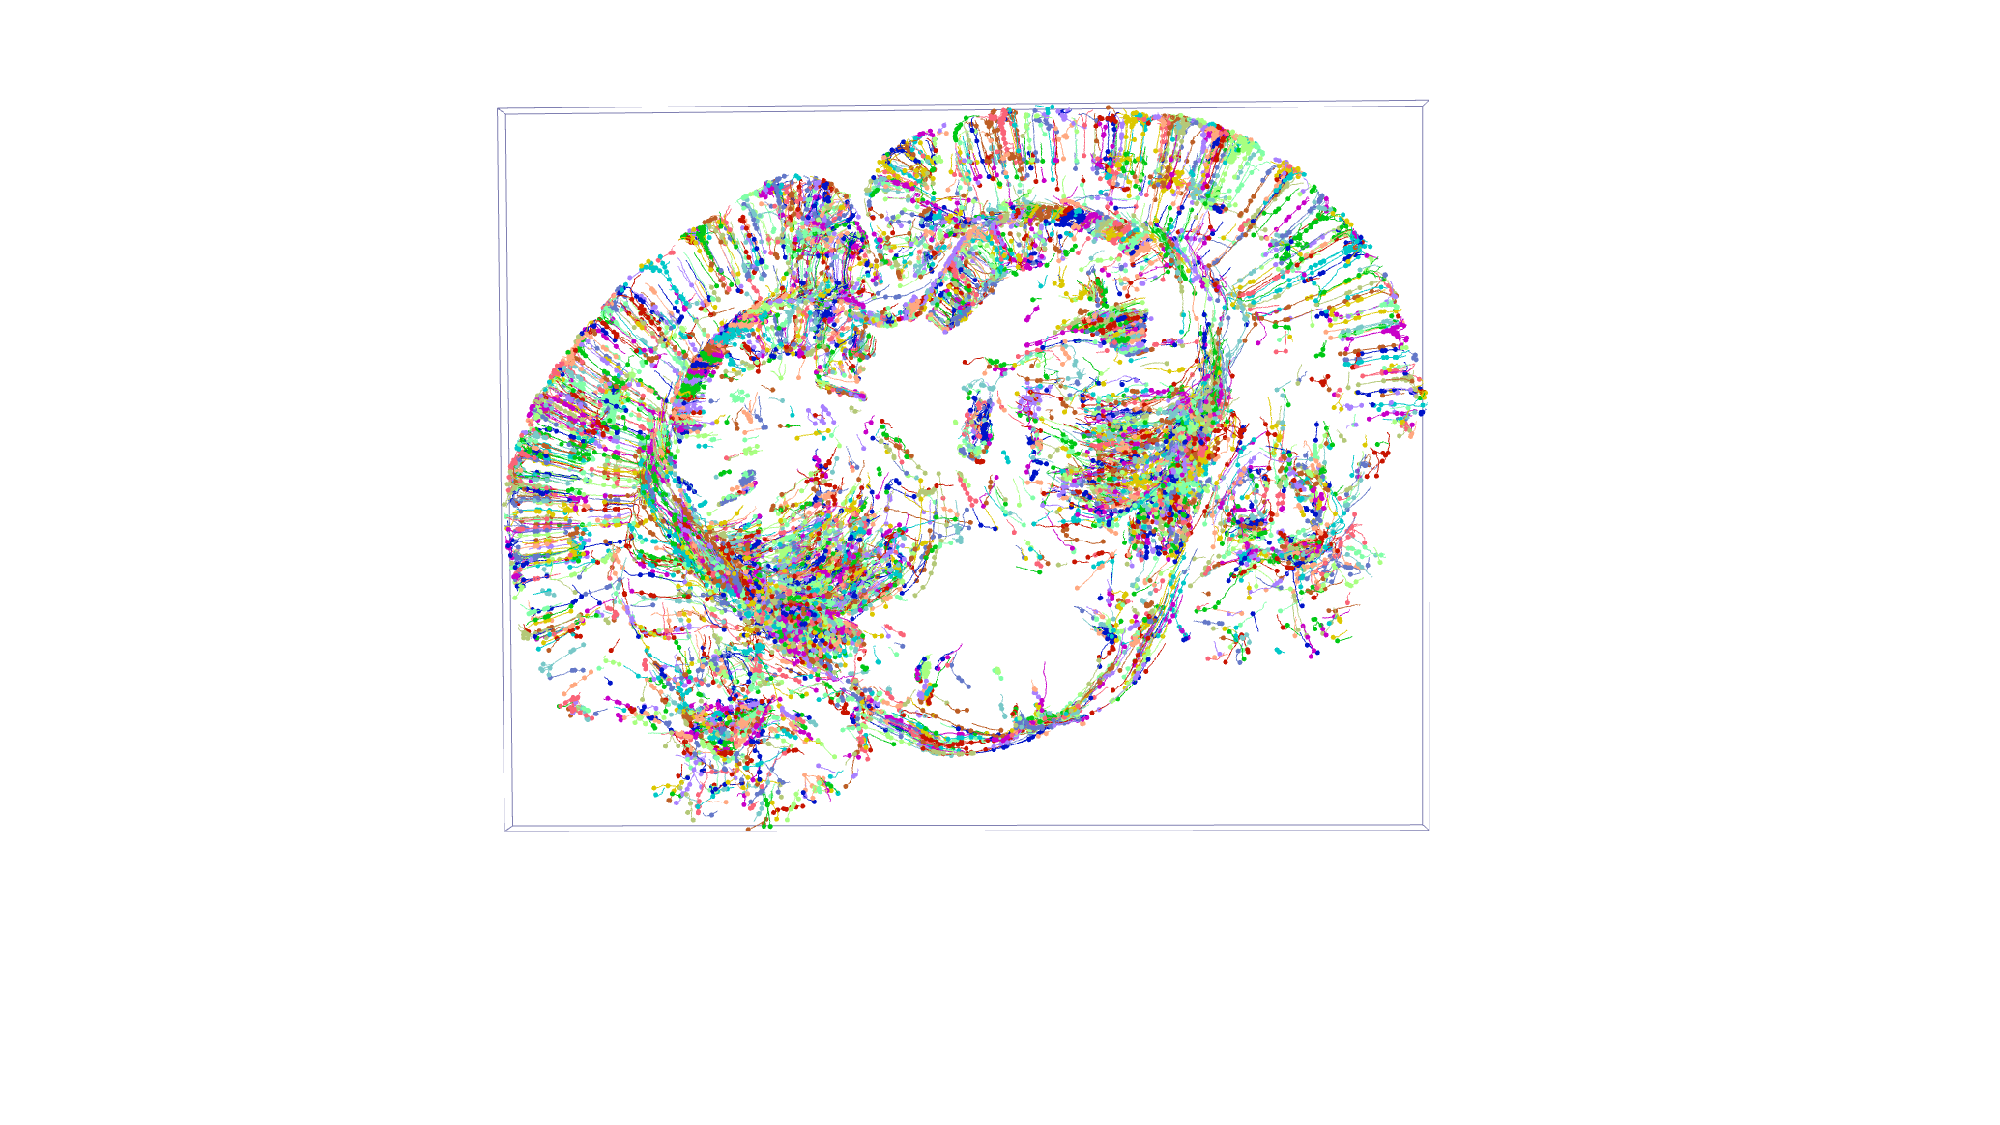
\includegraphics[width=1\columnwidth]{./Illustrations/brain_slice.pdf}
	\caption{The reconstruction result of neuronal populations in a large-scale 3D mouse brain slice using our UltraNPR method.}
	\label{fig:reconstruct_brain}
\end{figure}


On the BigNeuron dataset, we compare with seven widely used tracing methods to validate the effectiveness of our proposed method.
They are APP2~\cite{Xiao2013}, MOST~\cite{Wu2014}, SmartTracing~\cite{Chen2015}, NGPST~\cite{Quan2015}, Li2017~\cite{Li2017}, TReMAP~\cite{Zhou2016} and FMST~\cite{Yang2019} respectively.
%
The four metrics, including precision, recall, F-score, and Jaccard, are used for comparison for most methods.
However, the implementation of most learning-based tracing methods, such as~\cite{Li2017}, are not available.
In order to compare with~\cite{Li2017}, we only compare the three evaluation metrics reported in \cite{Li2017} on the same test data.
%
The three metrics defined in~\cite{Peng2010a} include the entire structure average (ESA), different structure average (DSA) and percentage of different structures (PDS).  
%
We evaluate the results obtained from different methods on the BigNeuron dataset in Table~\ref{table:compare_BigNeuron}.
The weighted averages of the ESA, DSA and PDS are calculated by setting the of each test block proportional to the neuron length identified in the corresponding manual annotation.
For these three scores, larger values indicate higher discrepancy between the tracing results and the manual reconstruction.
%
Fig.~\ref{fig:compare_BigNeuron} shows the reconstructed neurons from two test images using different methods.
%
From Table~\ref{table:compare_BigNeuron}, we can see that our method outperforms other methods on the BigNeuron dataset.
Though APP2~\cite{Xiao2013} achieves the highest precision, a large portion of subtle neurites are missing, as shown in Fig.~\ref{fig:compare_BigNeuron}.
%
Comparing with \cite{Li2017}, our PLNPR achieves comparable performance.
%
However, our method does not require any manual annotations to train the deep segmentation network.
With ever-increasing number of unlabeled neuron datasets are collected, our method could utilize them to further improve the performance of neuron reconstruction.



\subsection{Evaluation of UltraNPR on a Mouse Brain Slice}
\label{sec:exp_UltraNPR}

%\subsubsection{Experimental Settings}
To reconstruct the dense neuron population from an ultra-scale image, we divide the entire image into blocks in size of $1120\times 2048\times 869$ considering the memory and computational efficiency of our PLNPR.
%
The overlap between adjacent blocks is set to be $300$ voxels along each dimension. 
The $\delta_{ovlp}$ is set to be 10 voxels.
The $\delta_{bound}$ is set to be 70 voxels and the $\delta_{pt}$ is set to be 10 voxels for neurite fusion in Sec.~\ref{sec:fusion}.
%
It took our UltraNPR about 34 hours for deep image segmentation, 1 hour for neuron reconstruction in blocks, and 10 hours for neurite fusion to reconstruct the dense neuron population from the entire image on a cluster computer with $64$ GB of working memory and 20 NVIDIA 1080Ti GPUs.
%
As shown in Fig.~\ref{fig:reconstruct_brain}, a neuronal population which consists of $5348$ neurons is successfully reconstructed in the brain slice.


Since it is infeasible to manually annotate the dense nueron population in an ultra-scale image, quantitative evaluation of the reconstruction performance is supported.
%
However, we select four adjacent large-scale image blocks to qualitatively compare our UltraNPR with two state-of-the-art methods, UltraTracer~\cite{Peng2017} and MEIT~\cite{Wang2018}, for large-scale neuron reconstruction.
%
Fig.~\ref{fig:reconstruct_blocks} shows the neuronal populations reconstructed results.
%
MEIT~\cite{Wang2018} is designed for tracing single neuron, without separating individual neurons. 
Moreover, it fails to reconstruct the subtle dendrites due to the noises and low contrast in our challenging image.
%
\xj{Another drawback of MEIT is that many parameters have to be carefully tuned to obtain satisfied results. More results under different parameters using MEIT are shown in our supplementary files. }
% 
UltraTracer~\cite{Peng2017} achieves better performance of neuronal population reconstruction from the large-scale image. 
However, for the local regions with low signal-noise-ratio, it fails to separate individual neurons and trace complete dendrites in a dense neuron population. 
In comparison, thanks to the signal enhancement by our deep network and block propagation designed for dense neurites, our UltraNPR is more robust to reconstruct a more complete neuronal population from the low-quality image while individual neurons are continuously and smoothly traced.
 

\begin{figure*}[t]
	\centering
	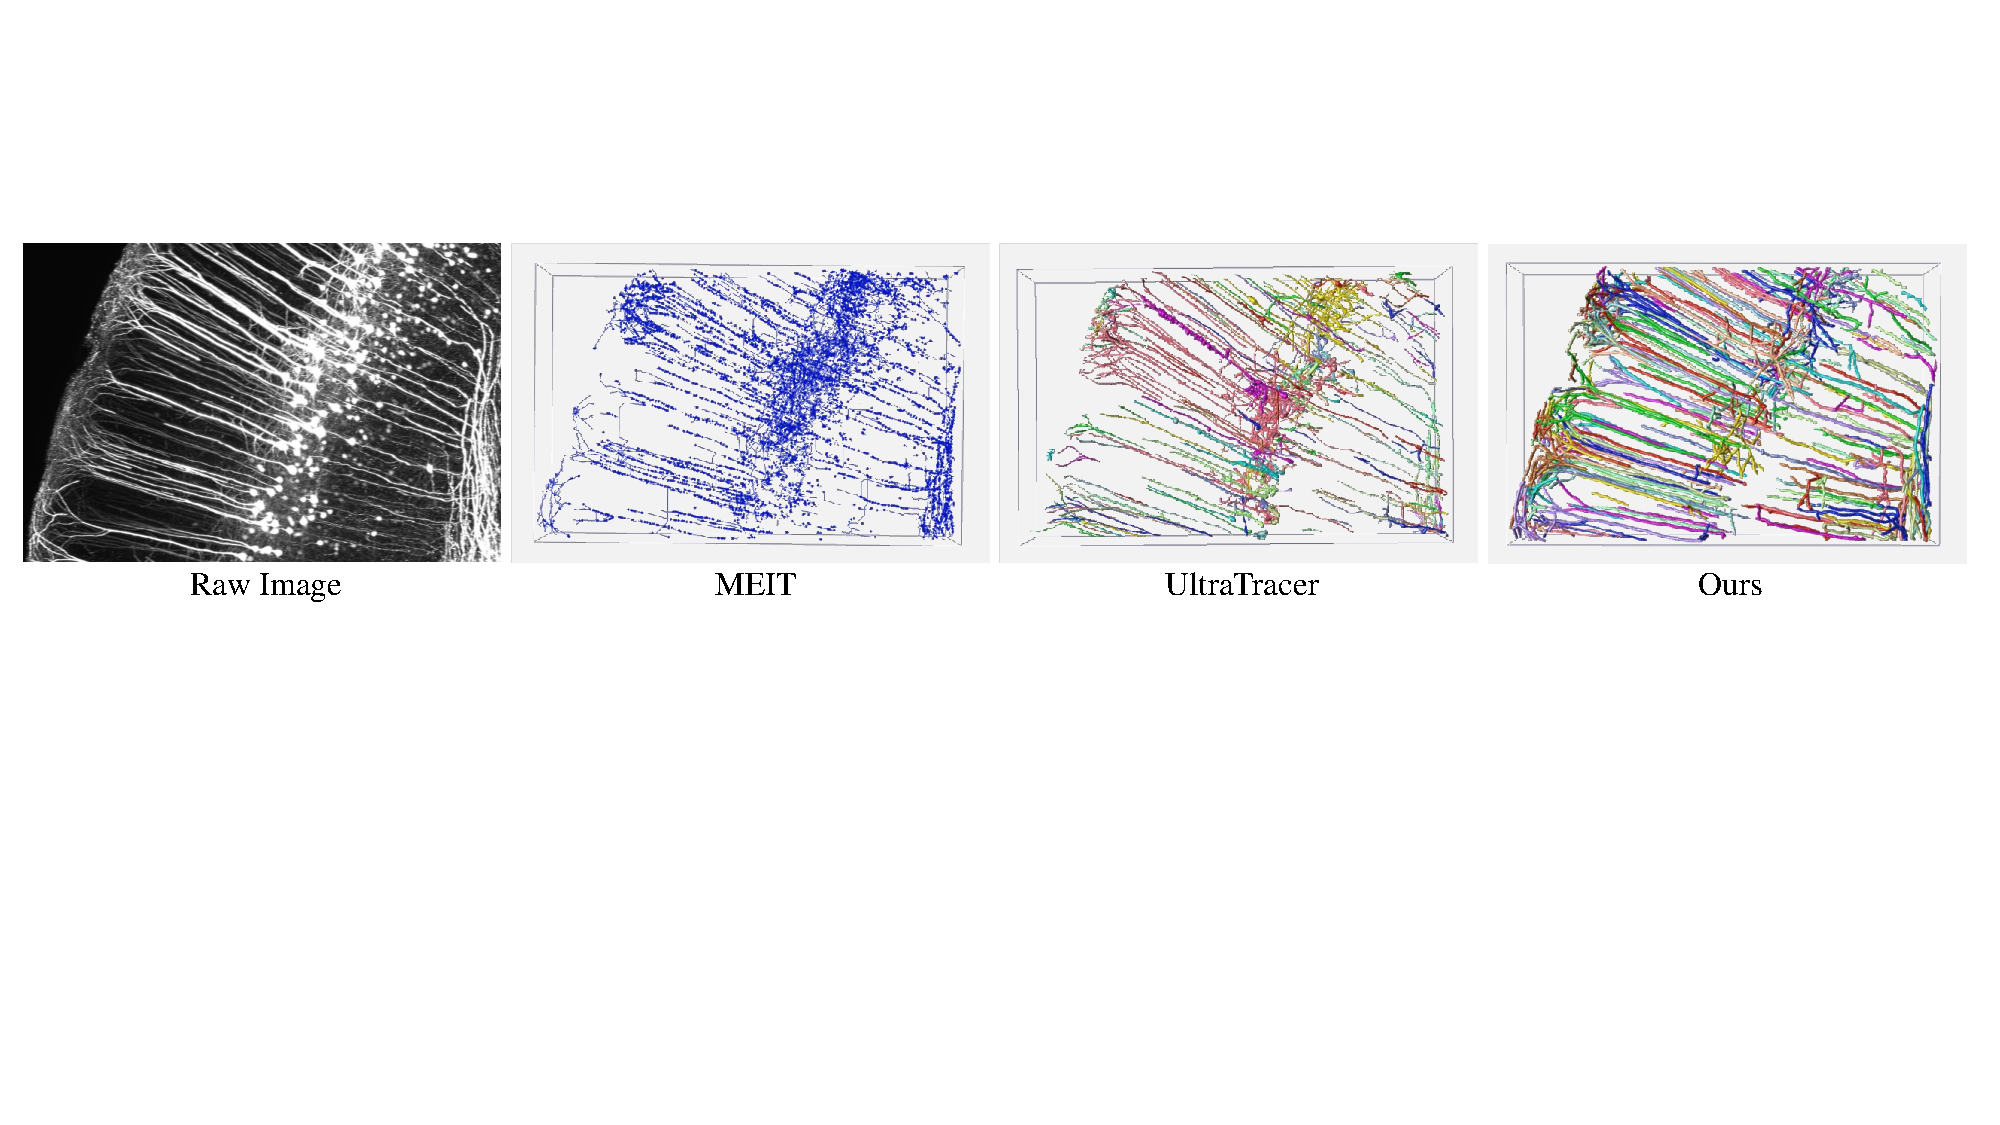
\includegraphics[width=\textwidth]{./Illustrations/comparison_ultranpr.pdf}
	\caption{Reconstruction results of dense neuronal populations from four adjacent large-scale blocks using UltraTracer~\cite{Peng2017}, MEIT~\cite{Wang2018} and our UltraNPR. \xj{The second row shows close-up views for a local region with dense neurites.} Our method reconstructs more complete and distinguishable neurons. 
	}
	\label{fig:reconstruct_blocks}
\end{figure*}



\begin{figure}[t]
	\centering
	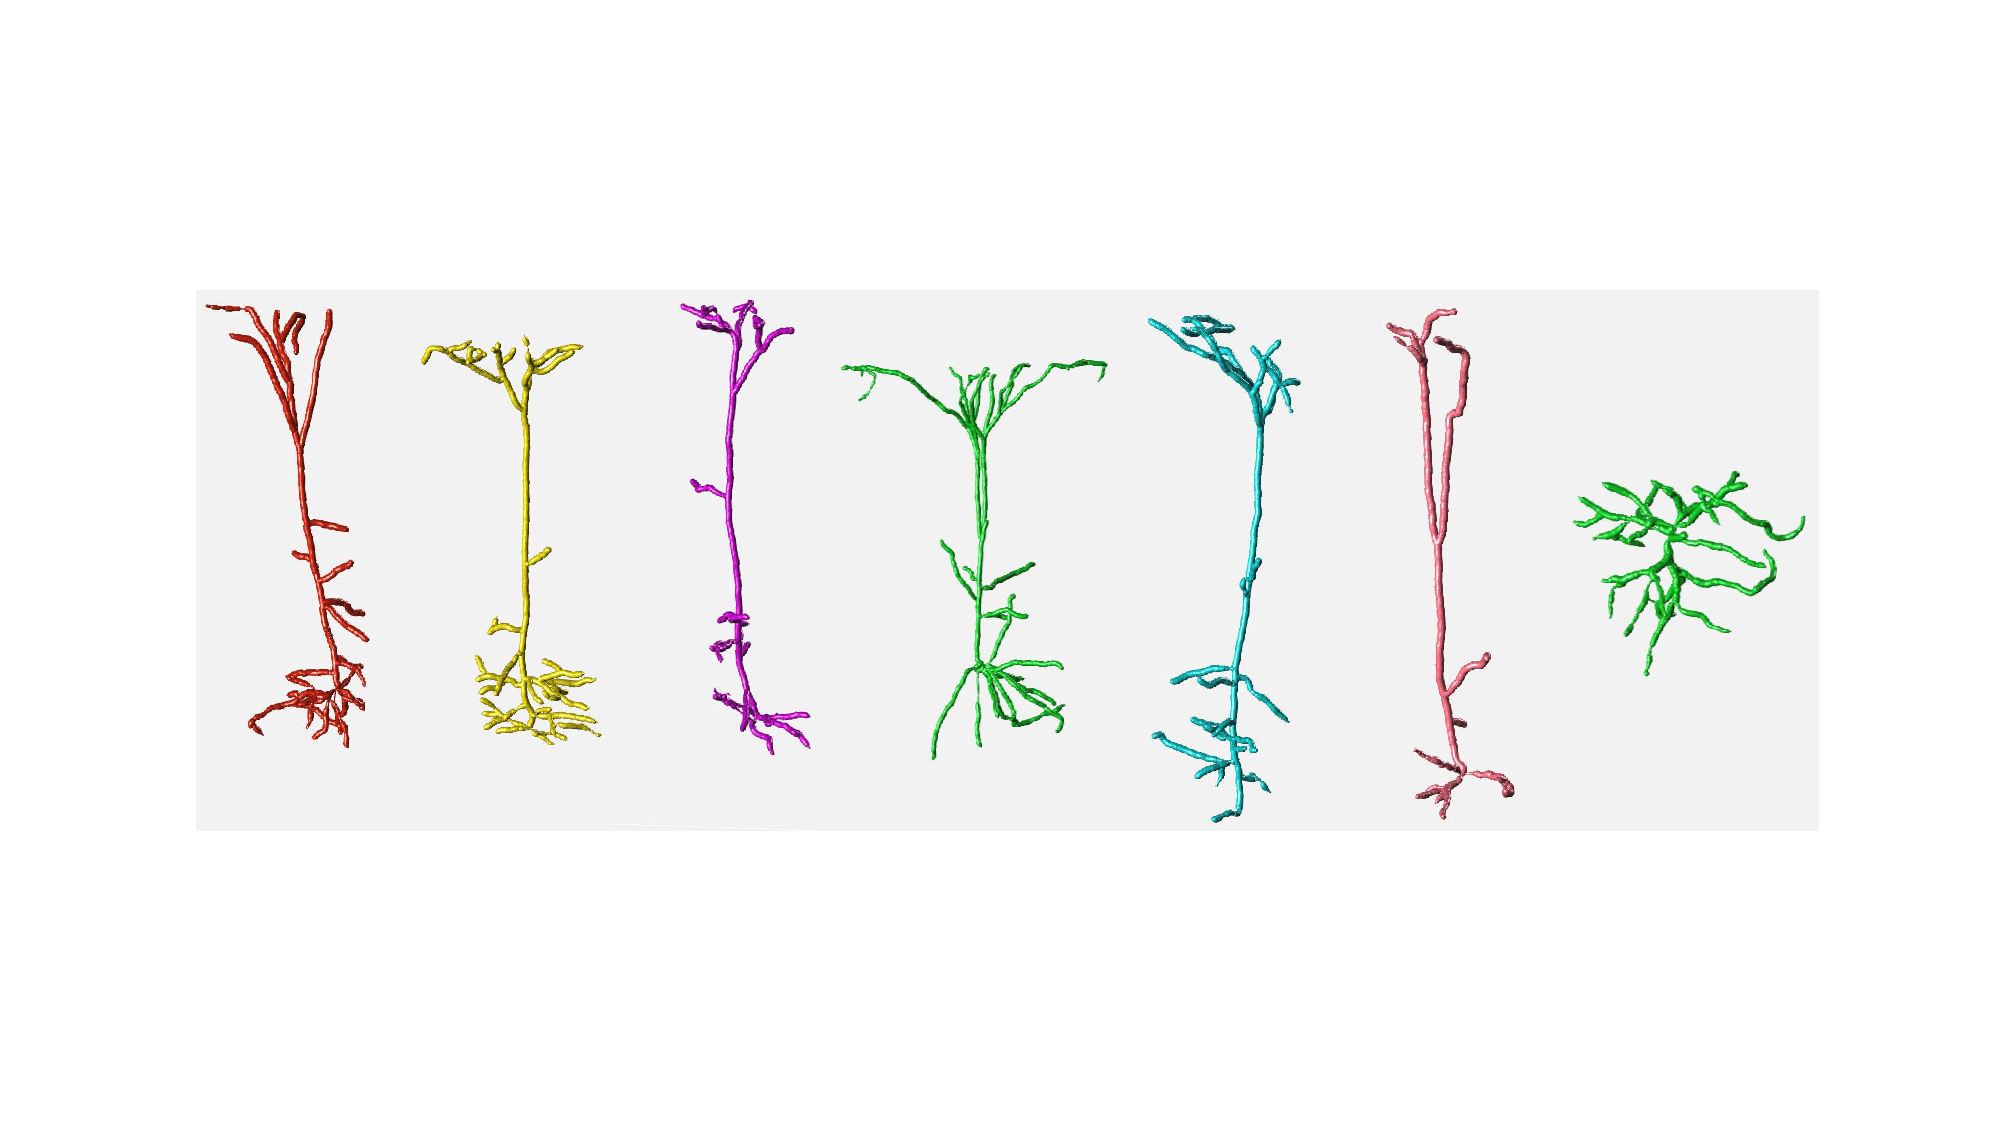
\includegraphics[width=\columnwidth]{./Illustrations/single_neurons4.pdf}
	\caption{Single neurons selected from the reconstructed neuronal populations in a mouse brain slice using our UltraNPR method.}
	\label{fig:single_neurons}
\end{figure}


Several neurons selected from the reconstructed neuronal population in the mouse brain slice are visualized in Fig.~\ref{fig:single_neurons}. 
We believe that these large-scale reconstructions provide detailed neuronal structures and will effectively support further neuronal morphology analysis in the whole brain. 
In summary, without any parameter-tuning and human interaction, our UltraNPR is capable of reconstructing dense neuronal populations from ultra-scale noisy OM images. 



\section{Conclusion}
\label{sec:conclusion}
In this work, we propose PLNPR, a progressive learning framework for neuronal population reconstruction from noisy and low-quality OM image blocks.
Without using any manual annotations, our PLNPR method takes advantage of neuron tracing techniques and deep segmentation networks, and makes them mutually complement and promote each other progressively.
We extensively validate the proposed PLNPR for neuron reconstruction and the results demonstrate the effectiveness and superiority of our method.
Integrating PLNPR with an efficient block-wise tracing and fusion strategy, our UltraNPR successfully reconstruct dense neuronal populations in a ultra-scale OM images of a mouse brain slice.
%
We construct a new dataset ``VISoR-40'' which consists of 40 OM image blocks for evaluation of neuronal population reconstruction.
This dataset is now available and we believe that it will facilitate further brain studies, including neuron counting, neuron reconstruction, neuron morphology analysis, and so on.

\section*{Acknowledgements}
This work was supported by the Natural Science Foundation of China [grant number 91732304]; and the Fundamental Research Funds for the Central Universities [grant numbers WK2380000002, WK3490000003].
 

\bibliographystyle{model2-names}\biboptions{authoryear}
\bibliography{NeuroSegRef}

\end{document}

